% Options for packages loaded elsewhere
\PassOptionsToPackage{unicode}{hyperref}
\PassOptionsToPackage{hyphens}{url}
\PassOptionsToPackage{dvipsnames,svgnames,x11names}{xcolor}
%
\documentclass[
doublespace,
  times]{anzsauth}

\usepackage{amsmath,amssymb}
\usepackage{iftex}
\ifPDFTeX
  \usepackage[T1]{fontenc}
  \usepackage[utf8]{inputenc}
  \usepackage{textcomp} % provide euro and other symbols
\else % if luatex or xetex
  \usepackage{unicode-math}
  \defaultfontfeatures{Scale=MatchLowercase}
  \defaultfontfeatures[\rmfamily]{Ligatures=TeX,Scale=1}
\fi
\usepackage{lmodern}
\ifPDFTeX\else  
    % xetex/luatex font selection
\fi
% Use upquote if available, for straight quotes in verbatim environments
\IfFileExists{upquote.sty}{\usepackage{upquote}}{}
\IfFileExists{microtype.sty}{% use microtype if available
  \usepackage[]{microtype}
  \UseMicrotypeSet[protrusion]{basicmath} % disable protrusion for tt fonts
}{}
\makeatletter
\@ifundefined{KOMAClassName}{% if non-KOMA class
  \IfFileExists{parskip.sty}{%
    \usepackage{parskip}
  }{% else
    \setlength{\parindent}{0pt}
    \setlength{\parskip}{6pt plus 2pt minus 1pt}}
}{% if KOMA class
  \KOMAoptions{parskip=half}}
\makeatother
\usepackage{xcolor}
\setlength{\emergencystretch}{3em} % prevent overfull lines
\setcounter{secnumdepth}{5}
% Make \paragraph and \subparagraph free-standing
\makeatletter
\ifx\paragraph\undefined\else
  \let\oldparagraph\paragraph
  \renewcommand{\paragraph}{
    \@ifstar
      \xxxParagraphStar
      \xxxParagraphNoStar
  }
  \newcommand{\xxxParagraphStar}[1]{\oldparagraph*{#1}\mbox{}}
  \newcommand{\xxxParagraphNoStar}[1]{\oldparagraph{#1}\mbox{}}
\fi
\ifx\subparagraph\undefined\else
  \let\oldsubparagraph\subparagraph
  \renewcommand{\subparagraph}{
    \@ifstar
      \xxxSubParagraphStar
      \xxxSubParagraphNoStar
  }
  \newcommand{\xxxSubParagraphStar}[1]{\oldsubparagraph*{#1}\mbox{}}
  \newcommand{\xxxSubParagraphNoStar}[1]{\oldsubparagraph{#1}\mbox{}}
\fi
\makeatother

\usepackage{color}
\usepackage{fancyvrb}
\newcommand{\VerbBar}{|}
\newcommand{\VERB}{\Verb[commandchars=\\\{\}]}
\DefineVerbatimEnvironment{Highlighting}{Verbatim}{commandchars=\\\{\}}
% Add ',fontsize=\small' for more characters per line
\usepackage{framed}
\definecolor{shadecolor}{RGB}{241,243,245}
\newenvironment{Shaded}{\begin{snugshade}}{\end{snugshade}}
\newcommand{\AlertTok}[1]{\textcolor[rgb]{0.68,0.00,0.00}{#1}}
\newcommand{\AnnotationTok}[1]{\textcolor[rgb]{0.37,0.37,0.37}{#1}}
\newcommand{\AttributeTok}[1]{\textcolor[rgb]{0.40,0.45,0.13}{#1}}
\newcommand{\BaseNTok}[1]{\textcolor[rgb]{0.68,0.00,0.00}{#1}}
\newcommand{\BuiltInTok}[1]{\textcolor[rgb]{0.00,0.23,0.31}{#1}}
\newcommand{\CharTok}[1]{\textcolor[rgb]{0.13,0.47,0.30}{#1}}
\newcommand{\CommentTok}[1]{\textcolor[rgb]{0.37,0.37,0.37}{#1}}
\newcommand{\CommentVarTok}[1]{\textcolor[rgb]{0.37,0.37,0.37}{\textit{#1}}}
\newcommand{\ConstantTok}[1]{\textcolor[rgb]{0.56,0.35,0.01}{#1}}
\newcommand{\ControlFlowTok}[1]{\textcolor[rgb]{0.00,0.23,0.31}{\textbf{#1}}}
\newcommand{\DataTypeTok}[1]{\textcolor[rgb]{0.68,0.00,0.00}{#1}}
\newcommand{\DecValTok}[1]{\textcolor[rgb]{0.68,0.00,0.00}{#1}}
\newcommand{\DocumentationTok}[1]{\textcolor[rgb]{0.37,0.37,0.37}{\textit{#1}}}
\newcommand{\ErrorTok}[1]{\textcolor[rgb]{0.68,0.00,0.00}{#1}}
\newcommand{\ExtensionTok}[1]{\textcolor[rgb]{0.00,0.23,0.31}{#1}}
\newcommand{\FloatTok}[1]{\textcolor[rgb]{0.68,0.00,0.00}{#1}}
\newcommand{\FunctionTok}[1]{\textcolor[rgb]{0.28,0.35,0.67}{#1}}
\newcommand{\ImportTok}[1]{\textcolor[rgb]{0.00,0.46,0.62}{#1}}
\newcommand{\InformationTok}[1]{\textcolor[rgb]{0.37,0.37,0.37}{#1}}
\newcommand{\KeywordTok}[1]{\textcolor[rgb]{0.00,0.23,0.31}{\textbf{#1}}}
\newcommand{\NormalTok}[1]{\textcolor[rgb]{0.00,0.23,0.31}{#1}}
\newcommand{\OperatorTok}[1]{\textcolor[rgb]{0.37,0.37,0.37}{#1}}
\newcommand{\OtherTok}[1]{\textcolor[rgb]{0.00,0.23,0.31}{#1}}
\newcommand{\PreprocessorTok}[1]{\textcolor[rgb]{0.68,0.00,0.00}{#1}}
\newcommand{\RegionMarkerTok}[1]{\textcolor[rgb]{0.00,0.23,0.31}{#1}}
\newcommand{\SpecialCharTok}[1]{\textcolor[rgb]{0.37,0.37,0.37}{#1}}
\newcommand{\SpecialStringTok}[1]{\textcolor[rgb]{0.13,0.47,0.30}{#1}}
\newcommand{\StringTok}[1]{\textcolor[rgb]{0.13,0.47,0.30}{#1}}
\newcommand{\VariableTok}[1]{\textcolor[rgb]{0.07,0.07,0.07}{#1}}
\newcommand{\VerbatimStringTok}[1]{\textcolor[rgb]{0.13,0.47,0.30}{#1}}
\newcommand{\WarningTok}[1]{\textcolor[rgb]{0.37,0.37,0.37}{\textit{#1}}}

\providecommand{\tightlist}{%
  \setlength{\itemsep}{0pt}\setlength{\parskip}{0pt}}\usepackage{longtable,booktabs,array}
\usepackage{calc} % for calculating minipage widths
% Correct order of tables after \paragraph or \subparagraph
\usepackage{etoolbox}
\makeatletter
\patchcmd\longtable{\par}{\if@noskipsec\mbox{}\fi\par}{}{}
\makeatother
% Allow footnotes in longtable head/foot
\IfFileExists{footnotehyper.sty}{\usepackage{footnotehyper}}{\usepackage{footnote}}
\makesavenoteenv{longtable}
\usepackage{graphicx}
\makeatletter
\newsavebox\pandoc@box
\newcommand*\pandocbounded[1]{% scales image to fit in text height/width
  \sbox\pandoc@box{#1}%
  \Gscale@div\@tempa{\textheight}{\dimexpr\ht\pandoc@box+\dp\pandoc@box\relax}%
  \Gscale@div\@tempb{\linewidth}{\wd\pandoc@box}%
  \ifdim\@tempb\p@<\@tempa\p@\let\@tempa\@tempb\fi% select the smaller of both
  \ifdim\@tempa\p@<\p@\scalebox{\@tempa}{\usebox\pandoc@box}%
  \else\usebox{\pandoc@box}%
  \fi%
}
% Set default figure placement to htbp
\def\fps@figure{htbp}
\makeatother

% The following \newcommands are intended for use in the *current*
% document ("protoType"). It is unlikely that authors of papers submitted
% to the Journal will need them.  (Of course if it turns out that you
% do indeed need them, then by all means feel free to make use of them.)
%%%%%%%%%%%%%%%%%%%%%%%%%%%%%%%%%%%%%%%%%%%%%%%%%%%%%%%%%%%%%%%%%%%%%%%%%%%%%%
\usepackage{lipsum}

\newcommand\BibTeX{{\rmfamily B\kern-.05em \textsc{i\kern-.025em b}\kern-.08em
T\kern-.1667em\lower.7ex\hbox{E}\kern-.125emX}}
\newcommand\MiKTeX{{\rmfamily M\kern-.05em \textsc{i\kern-.025em K}\kern-.08em
T\kern-.1667em\lower.7ex\hbox{E}\kern-.125emX}}
\newcommand\PracTeX{{\rmfamily P\kern-.05em \textsc{r\kern-.025em a\kern-.025em
c}\kern-.08em
T\kern-.1667em\lower.7ex\hbox{E}\kern-.125emX}}
%%%%%%%%%%%%%%%%%%%%%%%%%%%%%%%%%%%%%%%%%%%%%%%%%%%%%%%%%%%%%%%%%%%%%%%%%%%%%%

\usepackage{pmboxdraw}
\makeatletter
\@ifpackageloaded{caption}{}{\usepackage{caption}}
\AtBeginDocument{%
\ifdefined\contentsname
  \renewcommand*\contentsname{Table of contents}
\else
  \newcommand\contentsname{Table of contents}
\fi
\ifdefined\listfigurename
  \renewcommand*\listfigurename{List of Figures}
\else
  \newcommand\listfigurename{List of Figures}
\fi
\ifdefined\listtablename
  \renewcommand*\listtablename{List of Tables}
\else
  \newcommand\listtablename{List of Tables}
\fi
\ifdefined\figurename
  \renewcommand*\figurename{Figure}
\else
  \newcommand\figurename{Figure}
\fi
\ifdefined\tablename
  \renewcommand*\tablename{Table}
\else
  \newcommand\tablename{Table}
\fi
}
\@ifpackageloaded{float}{}{\usepackage{float}}
\floatstyle{ruled}
\@ifundefined{c@chapter}{\newfloat{codelisting}{h}{lop}}{\newfloat{codelisting}{h}{lop}[chapter]}
\floatname{codelisting}{Listing}
\newcommand*\listoflistings{\listof{codelisting}{List of Listings}}
\makeatother
\makeatletter
\makeatother
\makeatletter
\@ifpackageloaded{caption}{}{\usepackage{caption}}
\@ifpackageloaded{subcaption}{}{\usepackage{subcaption}}
\makeatother

\usepackage[]{natbib}
\bibliographystyle{anzsj}
\usepackage{bookmark}

\IfFileExists{xurl.sty}{\usepackage{xurl}}{} % add URL line breaks if available
\urlstyle{same} % disable monospaced font for URLs
\hypersetup{
  pdftitle={Automated Residual Plot Assessment with the R Package autovi and Shiny App autovi.web},
  pdfauthor={Weihao Li; Dianne Cook; Emi Tanaka; Susan VanderPlas; Klaus Ackermann},
  pdfkeywords={initial data analysis, statistical graphics, data
visualization, visual inference, computer vision, machine
learning, hypothesis testing, regression analysis},
  colorlinks=true,
  linkcolor={blue},
  filecolor={Maroon},
  citecolor={Blue},
  urlcolor={Blue},
  pdfcreator={LaTeX via pandoc}}

\usepackage{moreverb}
\usepackage{url}
\usepackage{grffile}
\usepackage[UKenglish]{isodate}

%%%%%%%%%%%%%%%%%%%%%%%%%%%%%%%%%%%%%%%%%%%%%%%%%%%%%%%%%%%%%%%%%%%%%%%%%%%%%%

% The year in the following may need to be updated!
\def\volumeyear{2024}

% The following command ("obviously") effects line numbering
% of the document.

\usepackage{lineno}
\linenumbers


\def\firstletters{\bgroup \catcode`-=10 \catcode`(=10 \filA}
\def\filA#1{\filB#1 {\end} }
\def\filB#1#2 {\ifx\end#1\egroup \else#1 \expandafter\filB\fi}

\runningheads{
Automated Residual Plot Assessment
}{
\firstletters{WEIHAO}LI, \firstletters{DIANNE}COOK, \firstletters{EMI}TANAKA, \firstletters{SUSAN}VANDERPLAS, AND  \firstletters{KLAUS}ACKERMANN
}

\title{Automated Residual Plot Assessment with the R Package autovi and
Shiny App autovi.web}
\usepackage{etoolbox}
\makeatletter
\providecommand{\subtitle}[1]{% add subtitle to \maketitle
  \apptocmd{\@title}{\par {\large #1 \par}}{}{}
}
\makeatother
\subtitle{ANZJS Quarto Template}

\author{
Weihao Li\addressnum{1},
Dianne Cook\addressnum{1},
Emi Tanaka\addressnum{2},
Susan VanderPlas\addressnum{3} and
Klaus Ackermann
\addressnum{1}
}
\affiliation{
Monash University,
The Australian National University and
University of Nebraska
}

\address{
\addressnum{1} Department of Econometrics and Business
Statistics, Monash University, Wellington Road, VIC 3800, Australia\\
\addressnum{2} Biological Data Science Institute, The Australian
National University, 46 Sullivan's Creek Road, ACT 2600, Australia\\
\addressnum{3} Department of Statistics, University of Nebraska, Hardin
Hall, 3310 Holdrege St Suite 340, Lincoln, NE 68583, United States\\
\hspace*{1ex} Email: \texttt{weihao.li@monash.edu}    
}


\date{2024}
\begin{document}

\begin{abstract}
Regression software is widely available, and there are many tools for
generating diagnostics and computing conventional residual tests.
However, the advice remains that the analyst should look at the residual
plot to check the fit. Perhaps, one of the reasons is that conventional
tests are too sensitive, strictly resulting in adequate models being
abandoned. Visually assess the strength of patterns in residual plots
requires human effort and suffers from the potential for inconsistent
decisions from different analysts. Using a lineup protocol, where the
residual plot is embedded among null plots, can help to alleviate
inconsistency, but requires even more human effort. This is the type of
task that in today's world might employ a robot to do the tedious work
for a human. Here we describe a new R package that includes a computer
vision model for automated assessment of residual plots, and an
accompanying Shiny app for ease of use. For a user-provided sample of
residuals, it predicts a measure of visual signal strength (VSS) and
provides a suite of supporting information to assist the analyst decide
on the appropriateness their model fit.
\end{abstract}

\keywords{initial data analysis; statistical graphics; data
visualization; visual inference; computer vision; machine
learning; hypothesis testing; regression analysis}
          
\ack{The author acknowledges that this template is based on the latex
template for Australian and New Zealand Journal of Statistics and
intersperses some text from the original prototype document.
\newline\vspace{1ex}\newline Opinions and attitudes expressed in this
document, which are not explicitly designated as Journal policy, are
those of the author and are \emph{not} necessarily endorsed by the
Journal, its editorial board, its publisher Wiley or by the Australian
Statistical Publishing Association Inc.}

\maketitle


\section{Introduction}\label{sec-autovi-introduction}

Regression analysis is a widely used statistical modeling technique
widely for data in many fields. There are a vast array of software for
conducting regression modeling and generating diagnostics. The package
\texttt{lmtest} \citep{lmtest} provides a suite of conventional tests.
The \texttt{stats} package \citep{stats} offers standard diagnostic
plots such as residuals vs.~fitted values, quantile-quantile (Q-Q)
plots, and residuals vs.~leverage plots. Packages like \texttt{jtools}
\citep{jtools}, \texttt{olsrr} \citep{olsrr}, \texttt{rockchalk}
\citep{rockchalk}, and \texttt{ggResidpanel} \citep{ggresidpanel}
provide similar graphical diagnostics, often with alternative aesthetics
or interactive features. All of these tools deliver the types of
diagnostic plots outlined in the classical text by
\citet{cook1982residuals}. The \texttt{ecostats} package
\citep{warton_global_2023} incorporates simulation envelopes into
residual plots, while \texttt{DHARMa} \citep{dharma} compares empirical
quantiles (0.25, 0.5, and 0.75) of scaled residuals to their theoretical
counterparts. \texttt{DHARMa} is particularly focused on detecting model
violations such as heteroscedasticity, incorrect functional forms, and
issues specific to generalized linear and mixed-effect models, like
over/under-dispersion. It also includes conventional test annotations to
help avoid misinterpretation.

However relying solely on subjective assessments of these plots can lead
to issues, such as over-interpreting random patterns as model
violations. \citet{li2024plot} demonstrated that visual methods using
the lineup protocol \citep{buja2009statistical} for assessing residuals
are more useful, and also perform more practically than conventional
tests due to their reduced sensitivity to minor departures. Packages
such as \texttt{nullabor} \citep{nullabor}, \texttt{HLMdiag}
\citep{loy2014hlmdiag}, and \texttt{regressinator}
\citep{regressinator}, enable users to compare observed residual plots
with samples from null distributions, helping to quantify the
significance of any detected patterns. However, the

However, as discussed in \citet{li2024automated}, the lineup protocol
has significant limitations in large-scale applications due dependence
on human labor. Thus a computer vision model was developed with an
associated statistical testing procedure to automate the assessment of
residual plots. This model takes a residual plot and a vector of
auxiliary variables (such as the number of observations) as inputs and
outputs the predicted visual signal strength (VSS). This strength
estimates the distance between the residual distribution of the fitted
regression model and the reference distribution assumed under correct
model specification.

To make the statistical testing procedure and trained computer vision
model widely accessible, we developed the R package \texttt{autovi}, and
a web interface, \texttt{autovi.web} to make it easy for users to
automatically read their residual plots with the trained computer vision
model.

The remainder of this paper is structured as follows:
Section~\ref{sec-autovi} provides a detailed documentation of the
\texttt{autovi} package, including its usage and infrastructure.
Section~\ref{sec-autovi-web} focuses on the \texttt{autovi.web}
interface, describing its design and usage, along with illustrative
examples. Finally, Section~\ref{sec-autovi-conclusion} presents the main
conclusions of this work.

\section{R package: autovi}\label{sec-autovi}

The main purpose of \texttt{autovi} is to provide rejection decisions
and \(p\)-values for testing the null hypothesis (\(H_0\)) that the
regression model is correctly specified. The package provides automated
interpretation of residual plots using computer vision. The name
\texttt{autovi} stands for \textbf{auto}mated \textbf{v}isual
\textbf{i}nference.

There are two ways to access the package, directly using R or through a
web interface, \texttt{autovi.web}. The web interface has the advantage
that it can be used without installing Python, R and the relevant
packages locally.

\subsection{Why use it}\label{sec-why}

Figure~\ref{fig-three-examples} shows three sets of plots of residuals
against fitted values. The simulated example in (a) might be interpreted
as a heteroscedastic pattern, however the automated reading would
predict this to have a visual signal strength (VSS) of 1.53, with a
corresponding \(p\)-value of 0.25. This means it is would be interpreted
as a good residual plot, that there is nothing in the data to indicate a
violation of model assumptions. Skewness in the predictor variables is
generating the apparent heteroscedasticity, where the smaller variance
in residuals at larger fitted values is due to smaller sample size only.
The Breusch-Pagan test \citep{breusch1979simple} for heteroscedasticity
would also not reject this as good residual plot.

The data in (b) is generated by fitting a linear model predicting
\texttt{mpg} based on \texttt{hp} using the \texttt{datasets::mtcars}.
It is a small data set, and there is a hint of nonlinear structure not
captured by the model. The automated plot reading would predict a VSS of
3.57, which has a \(p\)-value less than 0.05. That is, the nonlinear
structure is most likely real, and indicates a problem with the model.
The conventional test, a Ramsey Regression Equation Specification Error
Test (RESET) \citep{ramsey1969tests} would also strongly detect the
nonlinearity.

The third example is generated using the \texttt{surreal} package
\citep{surreal} where structured residuals are hidden in data, to be
revealed if the correct model is specified. Here a quote based on Tukey
is used as the residual structure ``visual summaries focus on unexpected
values''. The automated plot reading predicts the VSS to be 5.87, with a
\(p\)-value less than 0.05. This structure is blindingly obvious
visually, but a RESET test for nonlinear structure would not report a
problem. (It would be detected by a Breusch-Pagan for heteroscedasticity
and also Shapiro-Wilk test \citep{shapiro1965analysis} for
non-normality.)

\begin{figure}

\centering{

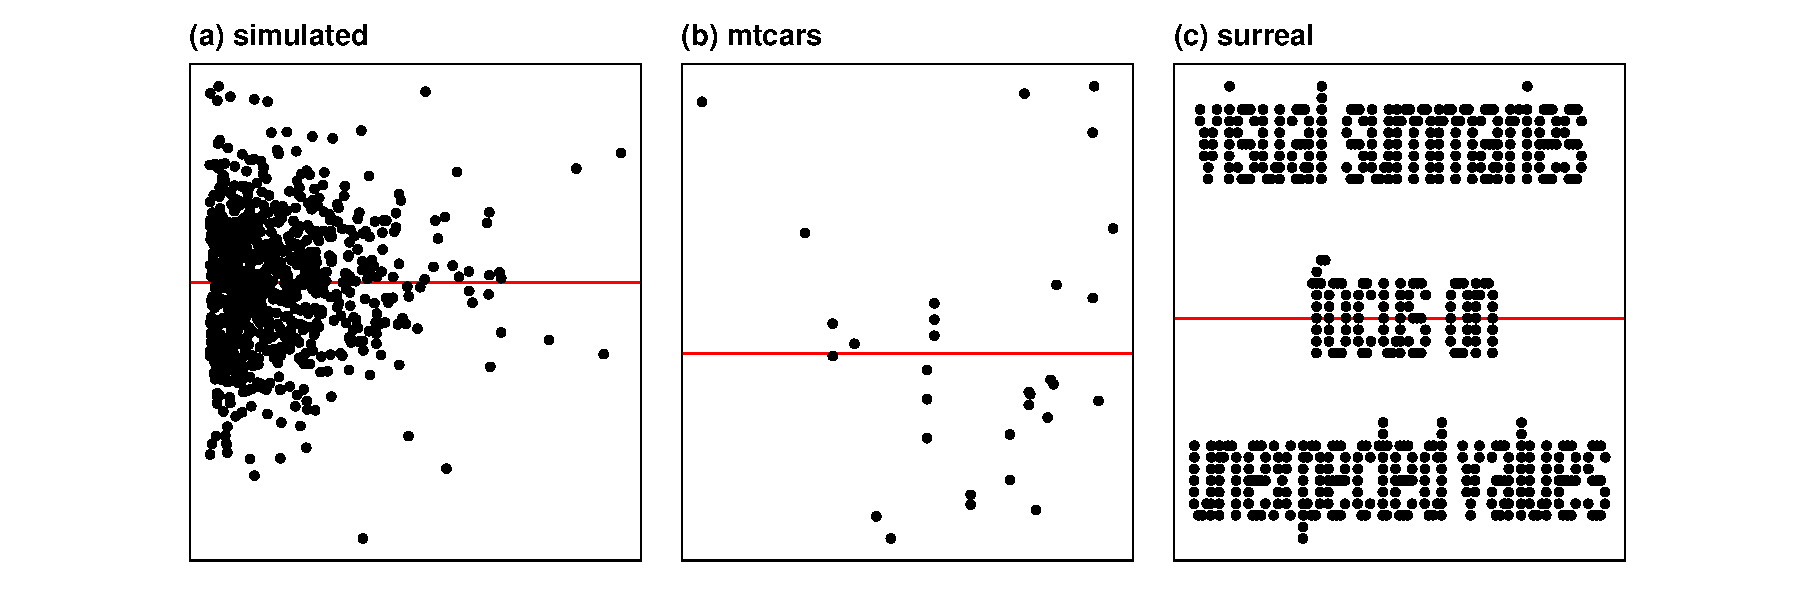
\includegraphics[width=1\linewidth,height=\textheight,keepaspectratio]{autovi_paper_files/figure-pdf/fig-three-examples-1.pdf}

}

\caption{\label{fig-three-examples}Reading residual plots can be a
difficult task, particular for students new to statistical modeling. The
autovi package makes it easier. Here are three examples of residual
plots, which may appear to have structure. According to autovi, the
visual signal strengths (VSS) of these three examples are approximately
(a) 1.53, (b) 3.57, (c) 5.87, resulting in (b), (c) being significant
violations of good residuals, but (a) is consistent with a good residual
plot.}

\end{figure}%

\subsection{Implementation}\label{sec-autovi-implementation}

The \texttt{autovi} package is built on the \texttt{bandicoot}
object-oriented programming (OOP) system \citep{bandicoot}, marking a
departure from R's traditional S3 generic system. This OOP architecture
enhances flexibility and modularity, allowing users to redefine key
functions through method overriding. While similar functionality could
be achieved using R's S3 system with generic functions, the OOP
framework offers a more structured and extensible foundation for the
package.

The \texttt{autovi} infrastructure effectively integrates multiple
programming languages and libraries into a comprehensive analytical
tool. It relies on five core libraries from Python and R, each playing a
critical role in the analysis pipeline. In Python, \texttt{pillow}
\citep{clark2015pillow} handles image processing tasks such as reading
and resizing PNG files of residual plots, then converting them into
input tensors for further analysis. The \texttt{TensorFlow}
\citep{abadi2016tensorflow} library, a key component of modern machine
learning, is used to predict the VSS of these plots through a
pre-trained convolutional neural network.

In the R environment, \texttt{autovi} utilizes several libraries.
\texttt{ggplot2} \citep{ggplot2} generates the initial residual plots,
saved as PNG files for visual input. The \texttt{cassowaryr}
\citep{mason2022cassowaryr} library computes scagnostics (scatter plot
diagnostics), providing numerical features that capture statistical
properties of the plots. These scagnostics complement the visual
analysis by offering quantitative metrics as secondary input to the
computer vision model. The \texttt{reticulate} \citep{reticulate}
package bridges R and Python, enabling seamless communication between
the two languages and supporting the integrated infrastructure.

\subsection{Installation}\label{installation}

The \texttt{autovi} package is available on CRAN. It is actively
developed and maintained, with the latest updates accessible on GitHub.
The code discussed in this paper is based on \texttt{autovi} version
0.4.1.

The package includes internal functions to check the current Python
environment used by the \texttt{reticulate} package. If the necessary
Python packages are not installed in the Python interpreter, an error
will be raised. If you want to select a specific Python environment, you
can do so by calling the \texttt{reticulate::use\_python()} function
before using the \texttt{autovi} package.

We recommend using the Shiny app \texttt{autovi.web} if encountering
installation problems.

\subsection{Numerical Summary}\label{sec-autovi-usage}

Three steps are needed to get an automated assessment of a set of
residuals and fitted values:

\begin{enumerate}
\def\labelenumi{\arabic{enumi}.}
\tightlist
\item
  Load the \texttt{autovi} package using the \texttt{library()}
  function.
\item
  Create a checker object with a linear regression model.
\item
  Call the \texttt{check()} method of the checker, which, by default,
  predicts the VSS for the true residual plot, 100 null plots, and 100
  bootstrapped plots, storing the predictions internally. A concise
  report of the check results is then printed.
\end{enumerate}

The code to do this is:

\begin{Shaded}
\begin{Highlighting}[]
\FunctionTok{library}\NormalTok{(autovi) }
\NormalTok{checker }\OtherTok{\textless{}{-}} \FunctionTok{residual\_checker}\NormalTok{(}\FunctionTok{lm}\NormalTok{(dist }\SpecialCharTok{\textasciitilde{}}\NormalTok{ speed, }\AttributeTok{data =}\NormalTok{ cars))}
\NormalTok{checker}\SpecialCharTok{$}\FunctionTok{check}\NormalTok{() }
\end{Highlighting}
\end{Shaded}

It produces the following summary:

\begin{verbatim}
\end{verbatim}

\begin{verbatim}
-- <AUTO_VI object>
Status:
 - Fitted model: lm
 - Keras model: UNKNOWN
    - Output node index: 1
 - Result:
    - Observed visual signal strength: 3.162 (p-value = 0.0396)
    - Null visual signal strength: [100 draws]
       - Mean: 1.274
       - Quantiles: 
          ╔═════════════════════════════════════════════════╗
          ║   25%    50%    75%    80%    90%    95%    99% ║
          ║0.8021 1.1109 1.5751 1.6656 1.9199 2.6564 3.3491 ║
          ╚═════════════════════════════════════════════════╝
    - Bootstrapped visual signal strength: [100 draws]
       - Mean: 2.786 (p-value = 0.05941)
       - Quantiles: 
          ╔══════════════════════════════════════════╗
          ║  25%   50%   75%   80%   90%   95%   99% ║
          ║2.452 2.925 3.173 3.285 3.463 3.505 3.652 ║
          ╚══════════════════════════════════════════╝
    - Likelihood ratio: 0.7275 (boot) / 0.06298 (null) = 11.55 
\end{verbatim}

The summary includes observed VSS of the true residual plot and
associated \(p\)-value of the automated visual test. The \(p\)-value is
the proportion of null plots (out of the total 100) that have VSS
greater than or equal to that of the true residual plot. The report also
provides sample quantiles of VSS for null samples and bootstrapped data
plots, providing more information about the sampling variability and a
likelihood of model violations. The likelihood is computed from the
proportion of values greater than the observed VSS in both the
bootstrapped data values and the simulated null values.

\subsection{Visual Summary}\label{sec-autovi-visual}

Users can visually inspect the original residual plot alongside a sample
null plot using \texttt{plot\_pair()} or a lineup of null plot
\texttt{plot\_lineup()}. This visual comparison can clarify why \(H_0\)
is either rejected or not, and help identify potential remedies.

\begin{Shaded}
\begin{Highlighting}[]
\NormalTok{checker}\SpecialCharTok{$}\FunctionTok{plot\_pair}\NormalTok{()}
\end{Highlighting}
\end{Shaded}

\begin{figure}[H]

\centering{

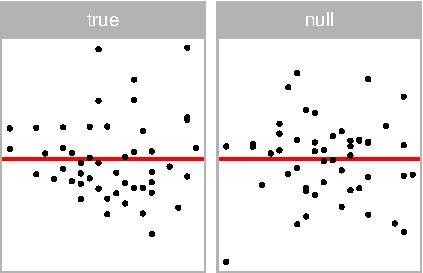
\includegraphics[width=0.6\linewidth,height=\textheight,keepaspectratio]{autovi_paper_files/figure-pdf/fig-plot-pair-1.pdf}

}

\caption{\label{fig-plot-pair}True plot alongside one null plot, for
quick comparison.}

\end{figure}%

The \texttt{plot\_pair()} method (Figure~\ref{fig-plot-pair}) displays
the true residual plot on the left and a single null plot on the right.
If a full lineup was shown, the true residual plot would be embedded in
a page of null plots. Users should look for any distinct visual patterns
in the true residual plot that are absent in the null plot. Running
these functions multiple times can help any visual suspicions, as each
execution generates new random null plots for comparison.

The package offers a straightforward visualization of the assessment
result through the \texttt{summary\_plot()} function.

\begin{Shaded}
\begin{Highlighting}[]
\NormalTok{checker}\SpecialCharTok{$}\FunctionTok{summary\_plot}\NormalTok{()}
\end{Highlighting}
\end{Shaded}

\begin{figure}[H]

\centering{

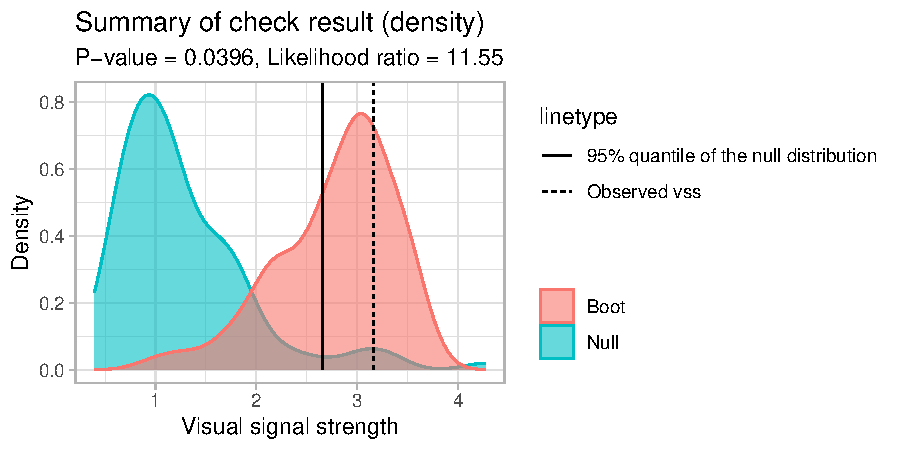
\includegraphics[width=1\linewidth,height=\textheight,keepaspectratio]{autovi_paper_files/figure-pdf/fig-summary-plot-1.pdf}

}

\caption{\label{fig-summary-plot}Summary plot comparing the densities of
VSS for bootstrapped residual samples (red) relative to VSS for null
plots (blue).}

\end{figure}%

In the result, shown in Figure~\ref{fig-summary-plot}, the blue area
represents the density of VSS for null residual plots, while the red
area shows the density for bootstrapped residual plots. The dashed line
indicates the VSS of the true residual plot, and the solid line marks
the critical value at a 95\% significance level. The \(p\)-value and the
likelihood ratio are displayed in the subtitle. The likelihood ratio
represents the ratio of the likelihood of observing the VSS of the true
residual plot from the bootstrapped distribution compared to the null
distribution.

Interpreting the plot involves several key aspects. If the dashed line
falls to the right of the solid line, it suggests rejecting the null
hypothesis. The degree of overlap between the red and blue areas
indicates similarity between the true residual plot and null plots;
greater overlap suggests more similarity. Lastly, the portion of the red
area to the right of the solid line represents the percentage of
bootstrapped models considered to have model violations.

This visual summary provides an intuitive way to assess the model's fit
and potential violations, allowing users to quickly grasp the results of
the automated analysis.

\subsection{Modularized Infrastructure}\label{sec-autovi-infrastructure}

\begin{figure}

\centering{

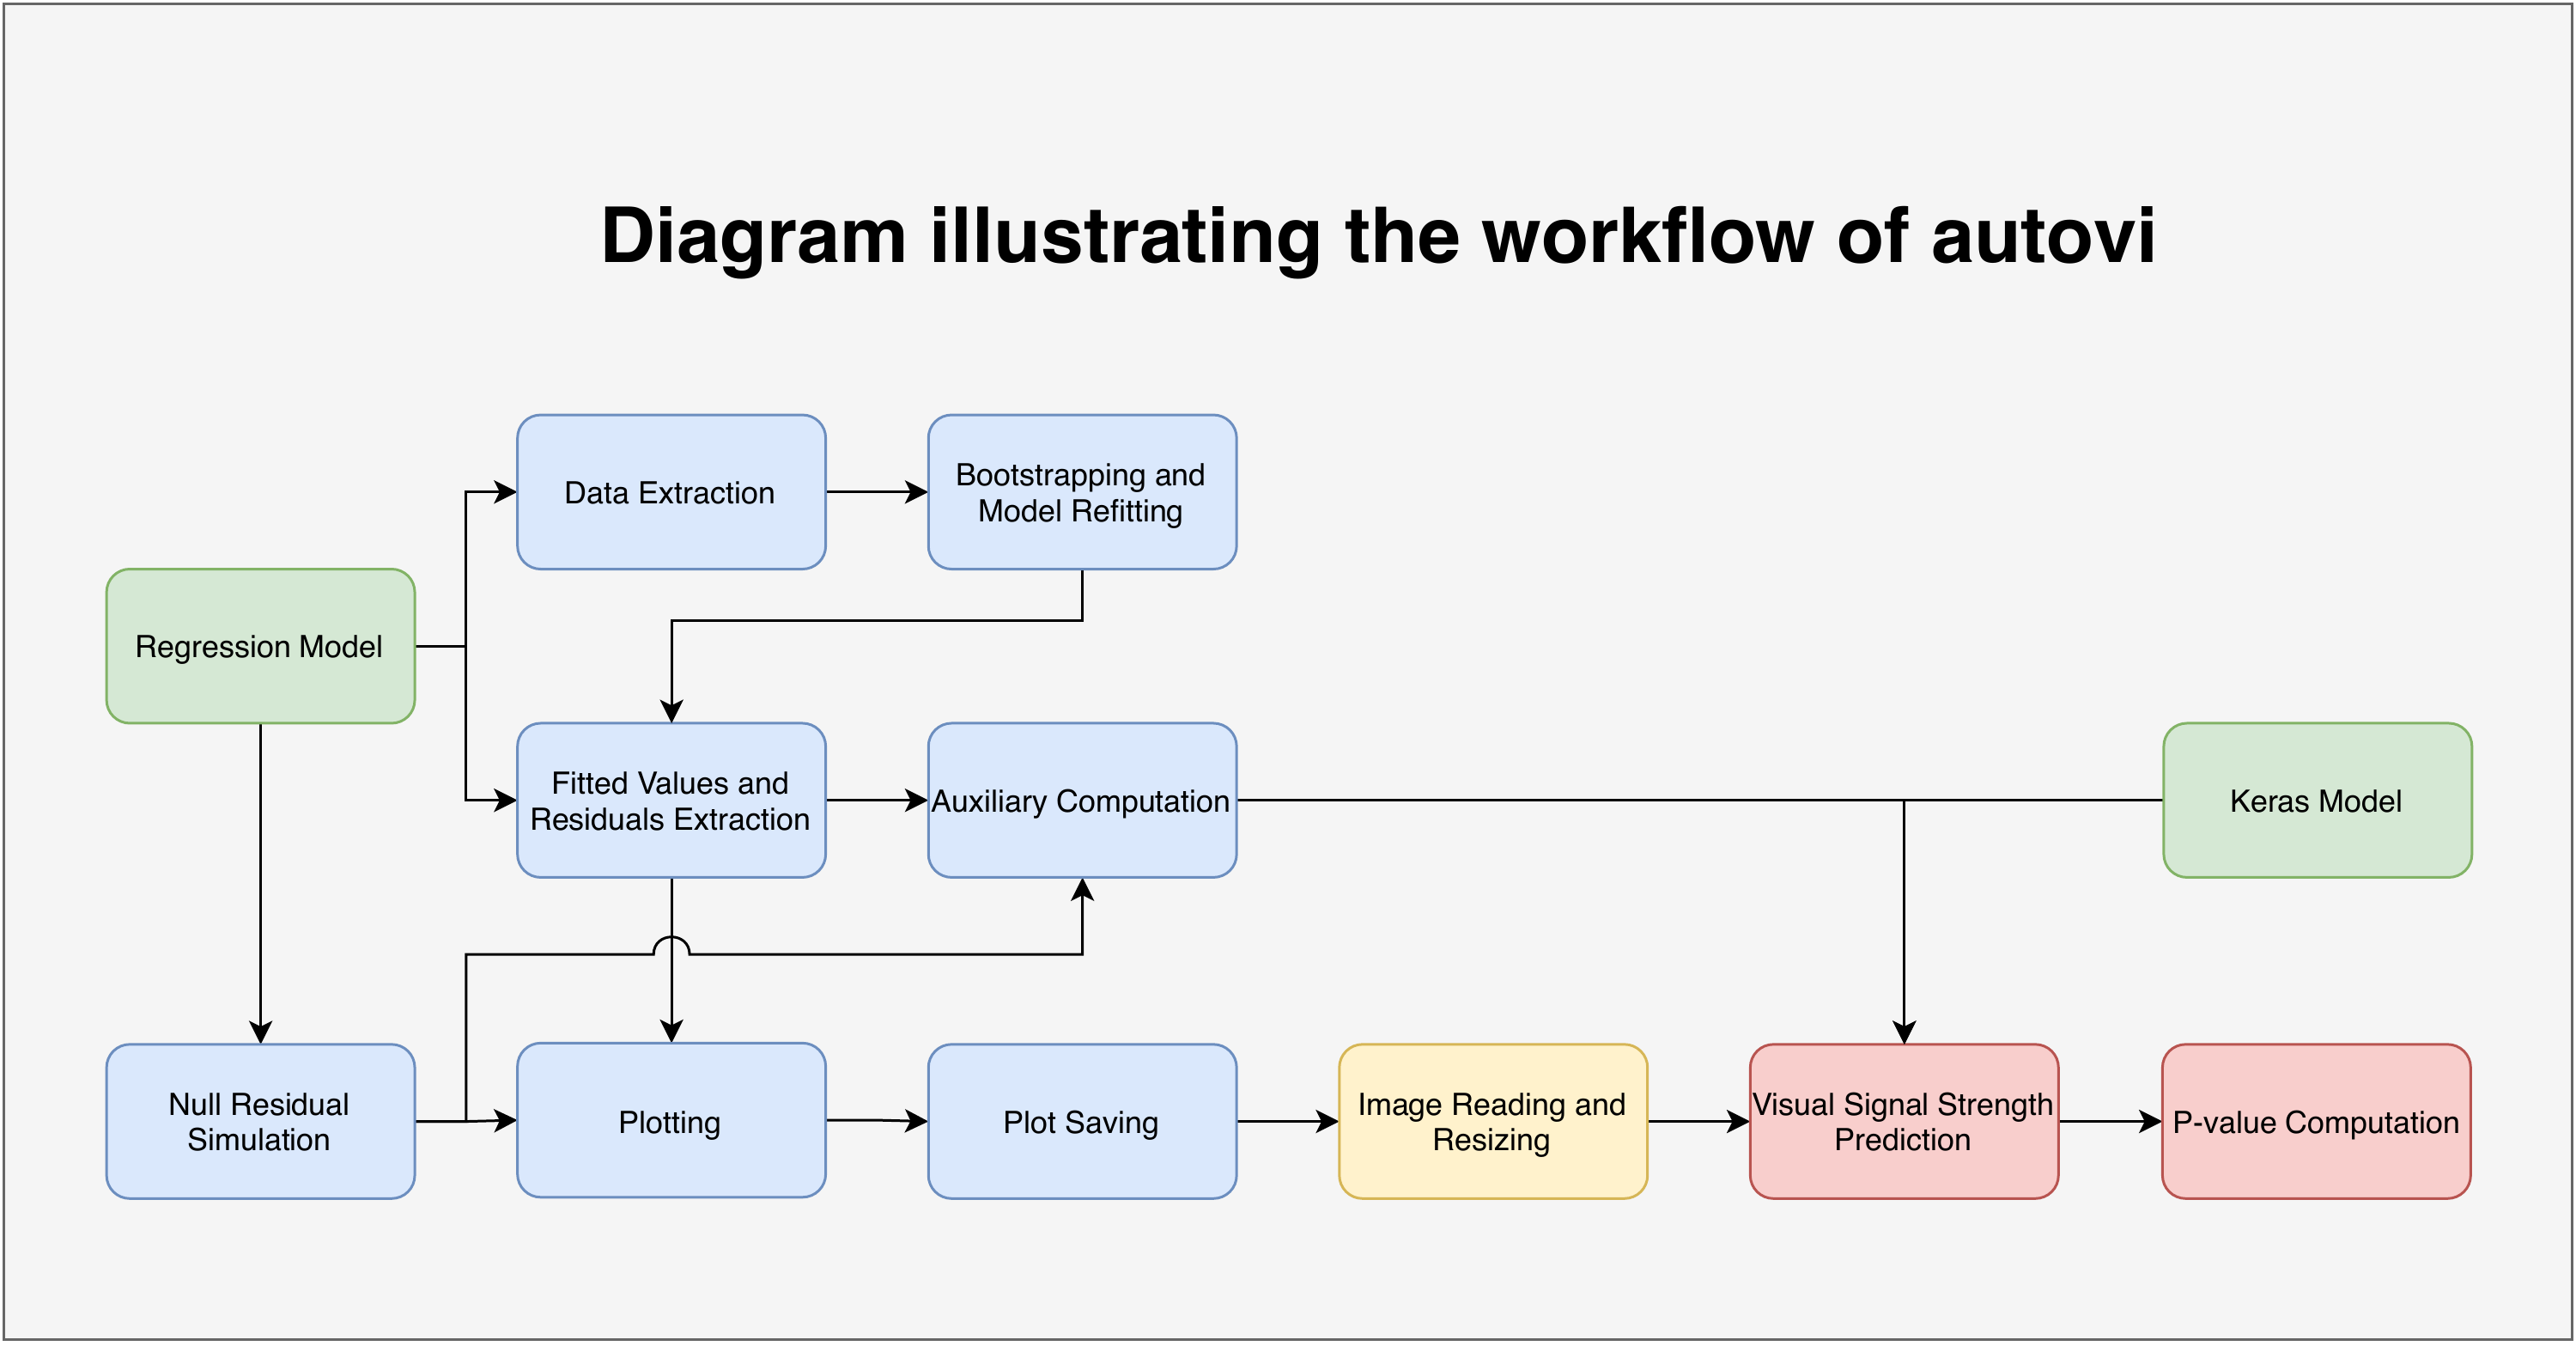
\includegraphics[width=1\linewidth,height=\textheight,keepaspectratio]{autovi_paper_files/figure-pdf/fig-autovi-diag-1.png}

}

\caption{\label{fig-autovi-diag}Diagram illustrating the infrastructure
of the R package autovi. The modules in green are primary inputs
provided by users. Modules in blue are overridable methods that can be
modified to accommodate users' specific needs. The module in yellow is a
pre-defined non-overridable method. The modules in red are primary
outputs of the package.}

\end{figure}%

The initial motivation for developing \texttt{autovi} was to create a
convenient interface for sharing the models described and trained in
\citet{li2024automated}. However, recognizing that the classical normal
linear regression model represents a restricted class of models, we
sought to avoid limiting the potential for future extensions, whether by
the original developers or other users. As a result, the package was
designed to function seamlessly with linear regression models with
minimal modification and few required arguments, while also
accommodating other classes of models through partial infrastructure
substitution. This modular and customizable design allows
\texttt{autovi} to handle a wide range of residual diagnostics tasks.

The infrastructure of \texttt{autovi} consists of ten core modules: data
extraction, bootstrapping and model refitting, fitted values and
residuals extraction, auxiliary computation, null residual simulation,
plotting, plot saving, image reading and resizing, VSS prediction, and
\(p\)-value computation. Each module is designed with minimal dependency
on the preceding modules, allowing users to customize parts of the
infrastructure without affecting its overall integrity. An overview of
this infrastructure is illustrated in Figure~\ref{fig-autovi-diag}.

The modules for VSS prediction and \(p\)-value computation are
predefined and cannot be overridden, although users can interact with
them directly through function arguments. Similarly, the image reading
and resizing module is fixed but will adapt to different Keras models by
checking their input shapes. The remaining seven modules are designed to
be overridable, enabling users to tailor the infrastructure to their
specific needs. These modules are discussed in detail on the software's
website.

\section{Web interface: autovi.web}\label{sec-autovi-web}

The \texttt{autovi.web} package extends the functionality of
\texttt{autovi} by offering a user-friendly web interface for automated
residual plot assessment. This eliminates the common challenges
associated with software installation, so users can avoid managing
Python environments or handling version requirements for R libraries.
The platform is cross-platform and accessible on various devices and
operating systems, making it suitable even for users without R
programming experience. Additionally, updates are managed centrally,
ensuring that users always have access to the latest features.

The \texttt{autovi.web} interface is available at
\url{autoviweb.netlify.app}. This section discusses the implementation
based on \texttt{autovi.web} version 0.1.0.

\subsection{Implementation}\label{implementation}

The package \texttt{autovi.web} is built using the \texttt{shiny}
\citep{shiny} and \texttt{shinydashboard} \citep{shinydashboard} R
packages. Hosted on the \href{https://www.shinyapps.io}{shinyapps.io}
domain, the application is accessible through any modern web browser.
The R packages \texttt{htmltools} \citep{htmltools} and
\texttt{shinycssloaders} \citep{shinycssloaders} are used to render
markdown documentation in shiny application, and for loading animations
for shiny widgets, respectively.

Determining the best way to implement the interface was difficult. In
our initial planning for \texttt{autovi.web}, we considered implementing
the entire web application using the \texttt{webr} framework
\citep{webr}, which would have allowed the entire application to run
directly in the user's browser. However, this approach was not feasible
at the time of writing this paper. The reason is that one of the R
packages \texttt{autovi} depends on the R package \texttt{splancs}
\citep{splancs}, which uses compiled Fortran code. A working Emscripten
\citep{zakai2011emscripten} version of this package, which would be
required for \texttt{webr}, was not available.

We also explored the possibility of implementing the web interface using
frameworks built on other languages, such as Python. However, server
hosting domains that natively support Python servers typically do not
have the latest version of R installed. Additionally, calling R from
Python is typically done using the \texttt{rpy2} Python library
\citep{rpy2}, but this approach can be awkward when dealing with
language syntax related to non-standard evaluation. Another option we
considered was renting a server where we could have full control, such
as those provided by cloud platforms like Google Cloud Platform (GCP) or
Amazon Web Services (AWS). However, correctly setting up the server and
ensuring a secure deployment requires significant expertise. Ultimately,
the most practical solution was to use the \texttt{shiny} and
\texttt{shinydashboard} frameworks, which are well-established in the R
community and offer a solid foundation for web application development.

The server-side configuration of \texttt{autovi.web} is carefully
designed to support its functionality. Most required Python libraries,
including \texttt{pillow} and \texttt{NumPy}, are pre-installed on the
server. These libraries are integrated into the Shiny application using
the \texttt{reticulate} package, which provides an interface between R
and Python.

Due to the resource allocation policy of shinyapps.io, the server enters
a sleep mode during periods of inactivity, resulting in the clearing of
the local Python virtual environment. Consequently, when the application
``wakes up'' for a new user session, these libraries need to be
reinstalled. While this ensures a clean environment for each session, it
may lead to slightly longer loading times for the first user after a
period of inactivity.

In contrast to \texttt{autovi}, \texttt{autovi.web} does not use the
native Python version of \texttt{TensorFlow}. Instead, it leverages
\texttt{TensorFlow.js}, a JavaScript library that allows the execution
of machine learning models directly in the browser. This choice enables
native browser execution, enhancing compatibility across different user
environments, and shifts the computational load from the server to the
client-side. \texttt{TensorFlow.js} also offers better scalability and
performance, especially when dealing with resource-intensive computer
vision models on shinyapps.io.

While \texttt{autovi} requires downloading the pre-trained computer
vision models from GitHub, these models in ``.keras'' file format are
incompatible with \texttt{TensorFlow.js}. Therefore, we extract and
store the model weights in JSON files and include them as extra
resources in the Shiny application. When the application initializes,
\texttt{TensorFlow.js} rebuilds the computer vision model using these
pre-stored weights.

To allow communication between \texttt{TensorFlow.js} and other
components of the Shiny application, the \texttt{shinyjs} R package is
used. This package allows calling custom JavaScript code within the
Shiny framework. The specialized JavaScript code for initializing
\texttt{TensorFlow.js} and calling \texttt{TensorFlow.js} for VSS
prediction is deployed alongside the Shiny application as additional
resources.

\subsection{Design}\label{sec-autovi-web-design}

\begin{figure}

\centering{

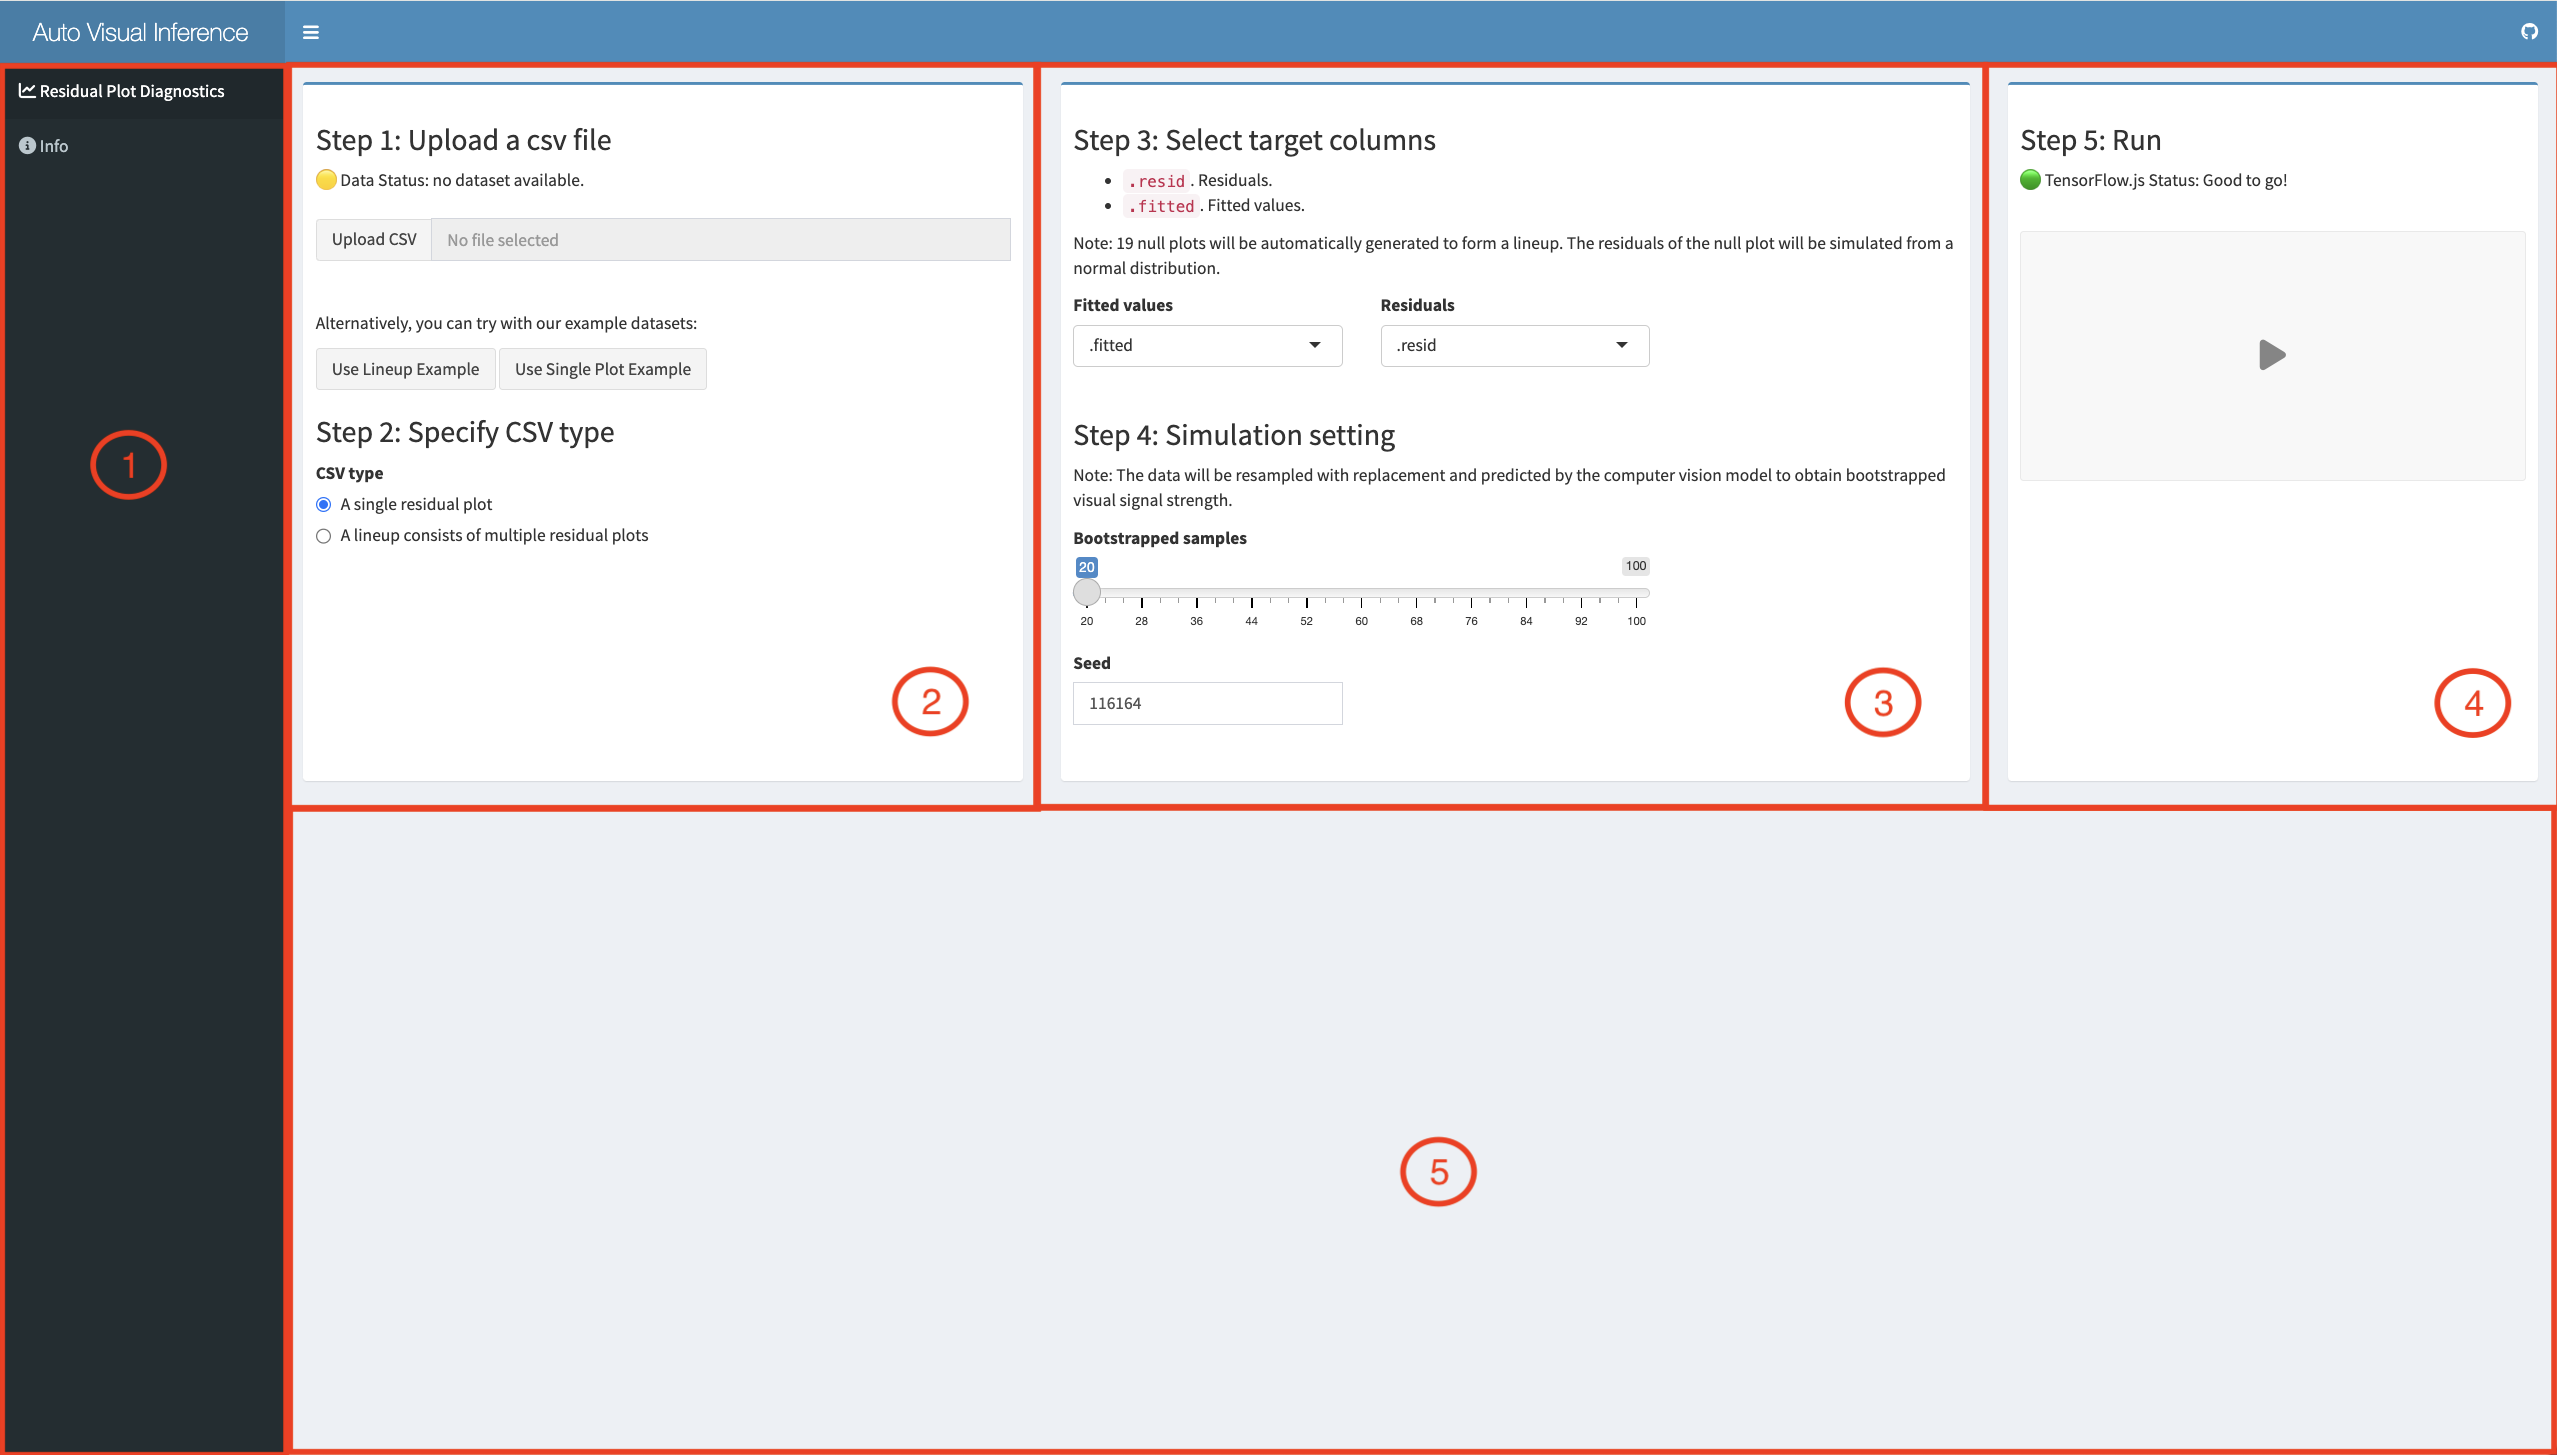
\includegraphics[width=1\linewidth,height=\textheight,keepaspectratio]{figures/autovi_web.png}

}

\caption{\label{fig-autovi-web}Overview of the \texttt{autovi.web}
graphical user interface (GUI). This default view may change based on
user interactions. Region 1 is the sidebar menu, containing the residual
assessment tab and the information tab. Region 2 is the data upload
panel, where users can provide a CSV file and specify the type of data
it contains. Region 3 includes dropdown menus for selecting the columns
to be analyzed, a slider to control the number of bootstrapping samples,
and a numeric input box for setting the simulation seed. Region 4
displays the initialization status and offers a button to start the
analysis. Region 5 is empty in the default view but will be populated
with results once the analysis is started.}

\end{figure}%

While the R package \texttt{autovi} aims to provide tools that can be
extended to broader visual inference applications, \texttt{autovi.web}
is only focus on providing a straightforward and clean user interface.
An overview of the graphical user interface of \texttt{autovi.web} is
provided in Figure~\ref{fig-autovi-web}. This is the default view of the
web application, and there are five regions that user can mainly
interact with. Region 1 of Figure~\ref{fig-autovi-web} is a sidebar menu
which can switch between the analysis page and the information page. The
analysis page is the focus of this section.

Region 2 of Figure~\ref{fig-autovi-web} is a panel for data uploading
and CSV type selection. Clicking the ``upload CSV'' button opens a
window where the user can select a file from their local system. The
data status displayed above the button provides information about the
number of rows and columns in the current dataset. Additionally, there
are two example datasets available beneath the ``upload CSV'' button:
one is a lineup example using a CSV file with three columns, and the
other is a single plot example using a CSV file with two columns. More
details about these example datasets are be discussed in
Section~\ref{sec-autovi-web-workflow}.

While the \texttt{autovi} package typically expects a fitted regression
model object provided by the user, this approach is impractical for a
web interface. Saving the R model object to the filesystem involves
extra steps and requires users to have specific knowledge, which does
not align with the goal of the web application. Moreover, the regression
model object may contain sensitive, non-shareable data, making it
unsuitable for uploading. Additionally, model objects are often
unnecessarily large, containing extra information not needed for
residual diagnostics. In contrast, a CSV file is easier to generate
using various software programs, not just R. CSV files are widely
accepted and can be easily viewed and modified using common desktop
applications like Excel. They are generally less sensitive than raw
data, as they exclude most information about the predictors.

The web application is designed to assess either a single residual plot
or a lineup of residual plots. Therefore, it accepts only two types of
CSV files: one with at least two columns representing the fitted values
and residuals of a single residual plot, and another with at least three
columns, where the additional column serves as the label or identifier
for a lineup of multiple residual plots. For a single residual plot, 19
null plots are generated by simulating normal random draws from a
distribution with the same variance as the original residual plot, and
comparisons are made with the original residual plot. For a lineup,
comparisons are made among the plots within the lineup. After uploading
the CSV file, the user must select the correct format to ensure the web
interface interprets the data correctly.

\begin{figure}

\centering{

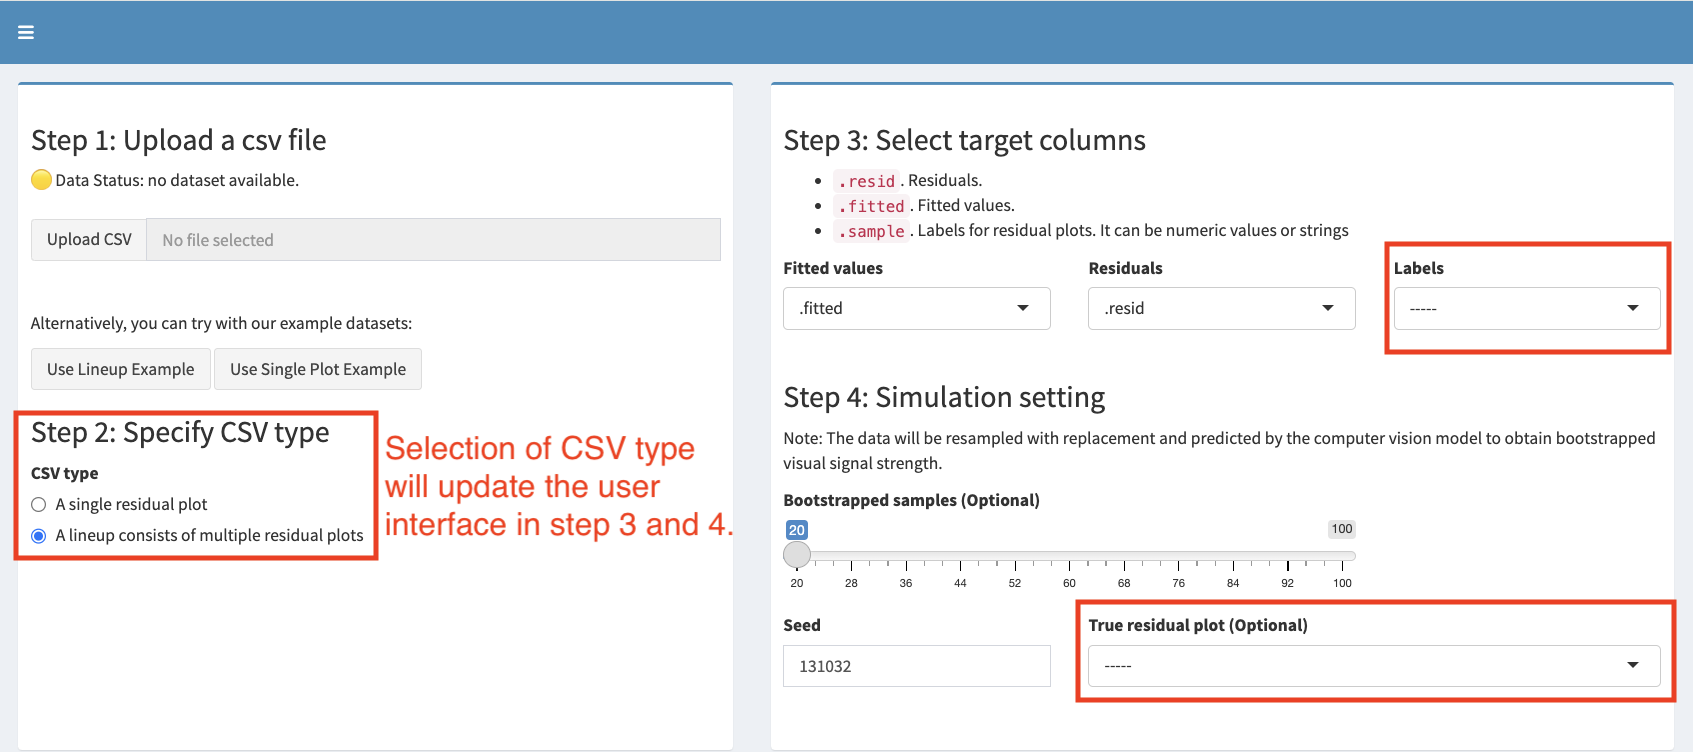
\includegraphics[width=1\linewidth,height=\textheight,keepaspectratio]{figures/autovi_web_type.png}

}

\caption{\label{fig-autovi-web-type}The panels for selecting target
columns and simulation settings are updated when a different CSV type is
selected in the left panel. Compared to Figure~\ref{fig-autovi-web},
where the CSV type is a single residual plot, choosing a CSV type that
includes a lineup of multiple residual plots adds a dropdown menu for
specifying a column for the residual plot identifier. Additionally, an
optional dropdown menu for specifying the true residual plot identifier
will appear under the simulation settings.}

\end{figure}%

Region 3 of Figure~\ref{fig-autovi-web} is a panel for column selection
and simulation settings. As shown in Figure~\ref{fig-autovi-web}, if the
CSV type is set to a single residual plot, there will be two dropdown
menus for specifying the columns for fitted values and residuals,
respectively. The default variable names for these columns are
\texttt{.fitted} and \texttt{.resid}. After uploading the CSV file, the
content of these dropdown menus will be updated to reflect the existing
columns in the dataset. As displayed in
Figure~\ref{fig-autovi-web-type}, for the CSV type that is a lineup of
multiple residual plots, an additional dropdown menu will appear for
specifying the column of residual plot labels. The default variable name
for this column is \texttt{.sample}. If this variable name does not
exist in the dataset, the dropdown menu will remain empty, allowing the
user to specify the correct column. The number of levels for each option
in this dropdown menu will be displayed to help avoid the selection of a
variable with too many levels, which could significantly slow down the
application due to extensive computation.

Under the simulation settings, there is a slider for specifying the
number of bootstrapped samples needed for the assessment. A higher value
on this slider will result in a more accurate bootstrap distribution
estimation, though it will require more computation time. The simulation
seed can be set in a numeric input box below the slider to control the
reproducibility of the assessment. By default, a random seed is set each
time the web page is refreshed. When the CSV type is a lineup of
multiple residual plots, an optional dropdown menu will appear next to
the simulation seed input box, allowing the user to specify an
identifier for the true residual plot. If no label is provided for the
true residual plot, the assessment will only estimate the VSS for each
residual plot in the lineup, without providing a \(p\)-value, as it
cannot be computed. Consequently, some result panels may be missing due
to insufficient information. This option is useful when the lineup
consists solely of null plots or if the user simply wants to obtain the
VSS for multiple residual plots.

Region 4 of Figure~\ref{fig-autovi-web} is the panel for triggering the
assessment. It contains a large play button to start the assessment.
Above the play button, a text message displays the status of
\texttt{TensorFlow.js}, allowing users to monitor whether the JavaScript
library and Keras model have been loaded correctly. The play button will
remain disabled until both the data status in Region 1 and the
\texttt{TensorFlow.js} status in Region 4 indicate that everything is
ready, with both showing a green status.

Once the play button is clicked, region 5 of Figure~\ref{fig-autovi-web}
will be populated with panels displaying the assessment results.
Generally, there will be four result panels, as shown in
Figure~\ref{fig-autovi-web-result} and
Figure~\ref{fig-autovi-web-result2}.

\begin{figure}

\centering{

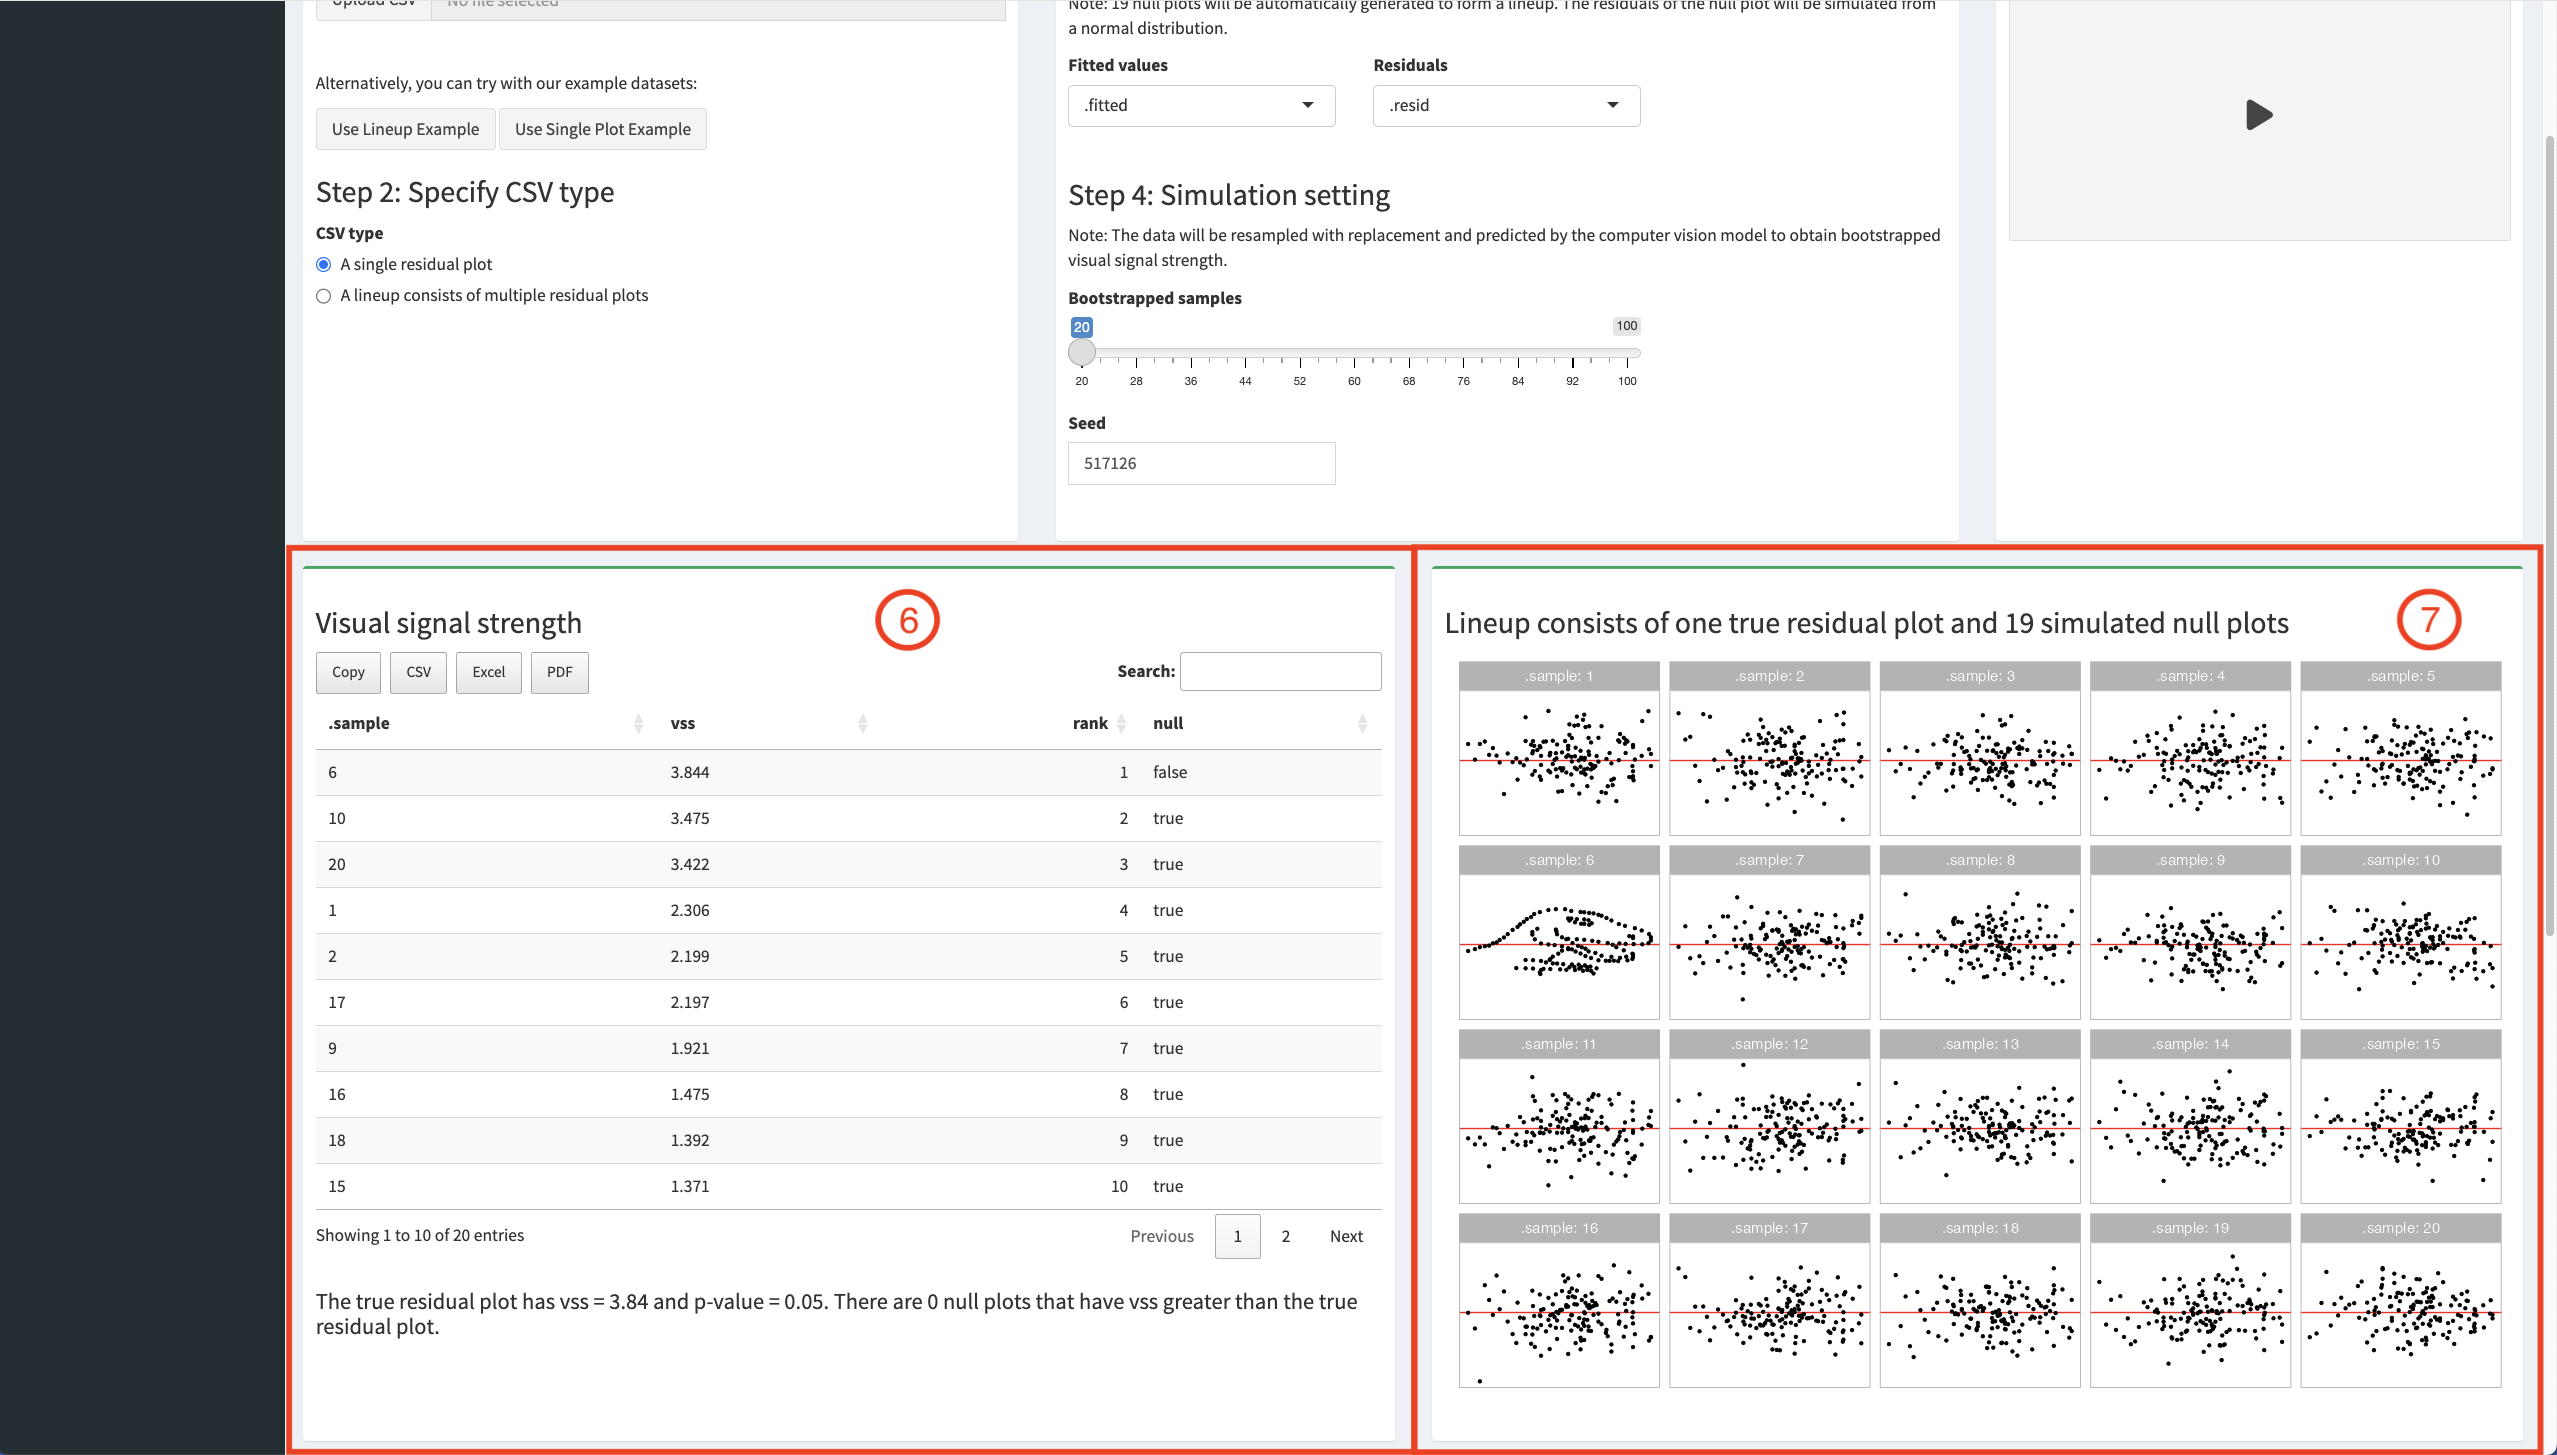
\includegraphics[width=1\linewidth,height=\textheight,keepaspectratio]{figures/autovi_web_result.png}

}

\caption{\label{fig-autovi-web-result}The first two panels of results
from the automated residual assessment are shown. The application
provides four results panels in total, and these screenshots display the
first two. In region 1, there is an interactive table detailing the VSS,
with a summary of the analysis provided in the paragraph below. Region 2
displays a lineup of residual plots.}

\end{figure}%

\begin{figure}

\centering{

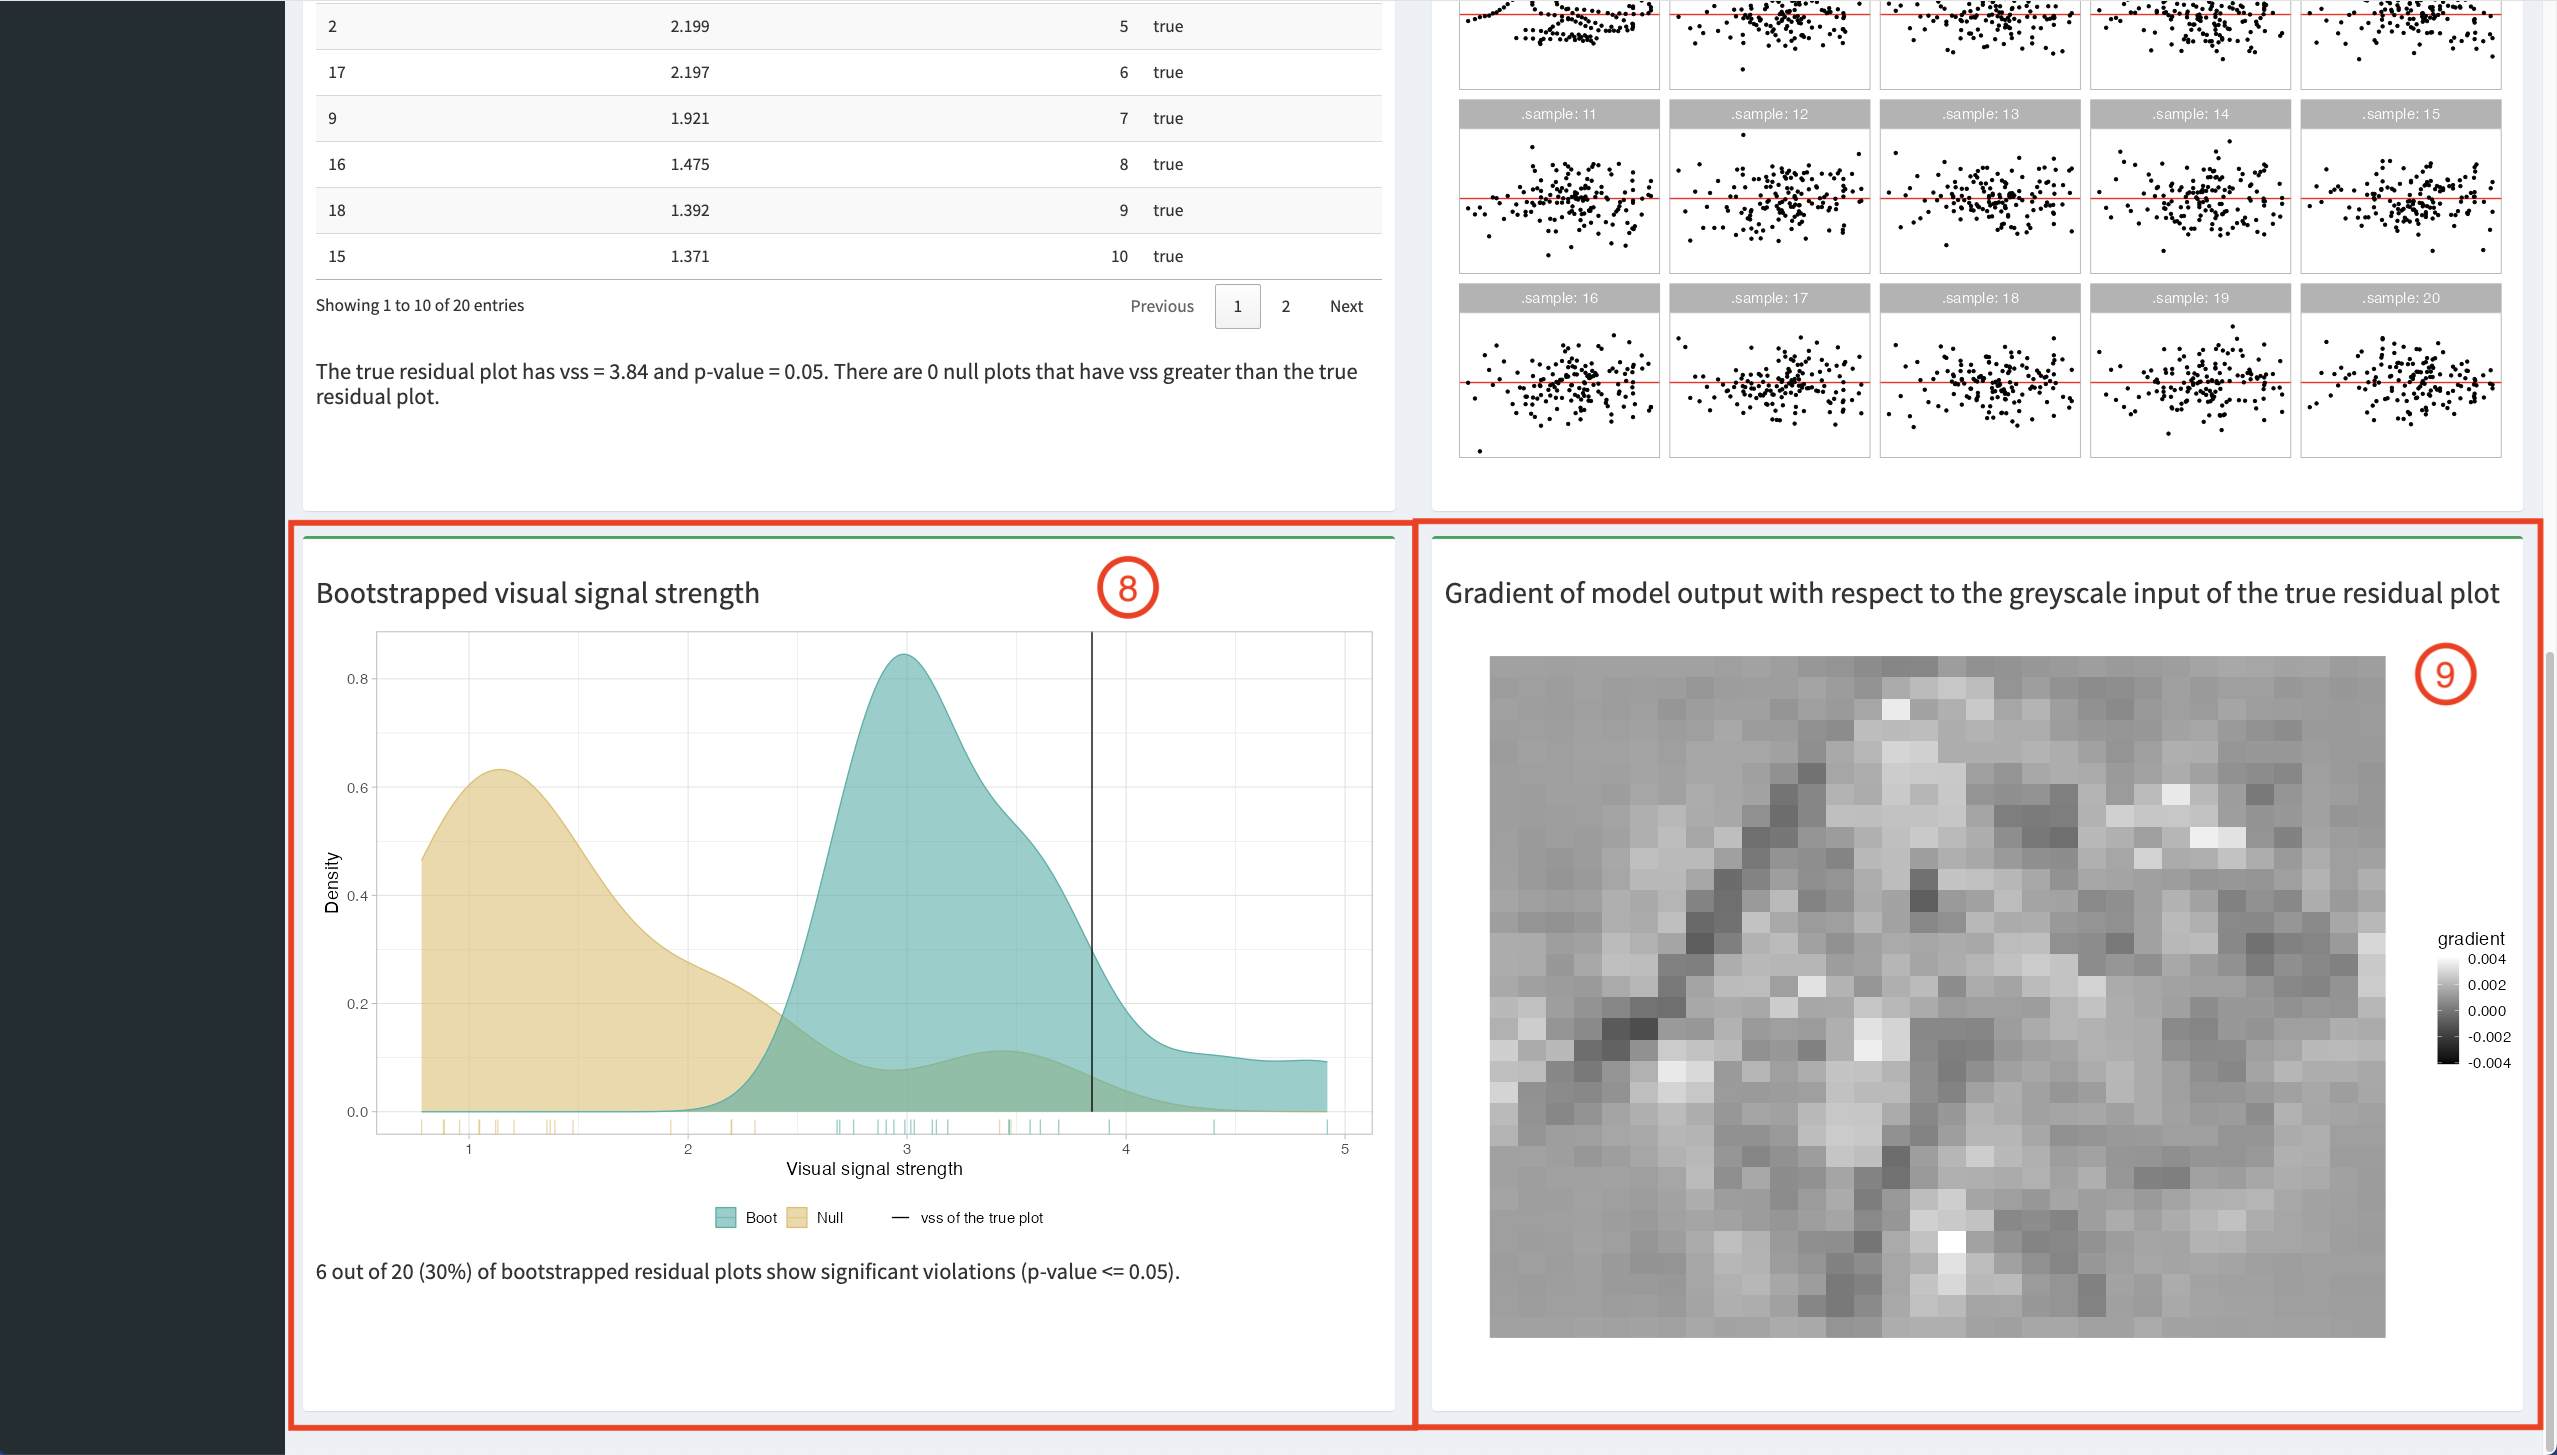
\includegraphics[width=1\linewidth,height=\textheight,keepaspectratio]{figures/autovi_web_result2.png}

}

\caption{\label{fig-autovi-web-result2}The last two panels of results
from the automated residual assessment are shown. The application
provides four results panels in total, and these screenshots display the
final two. Region 1 presents a density plot comparing the bootstrapped
VSS with the null VSS. Region 2 includes an attention map of the true
residual plot.}

\end{figure}%

\begin{figure}

\centering{

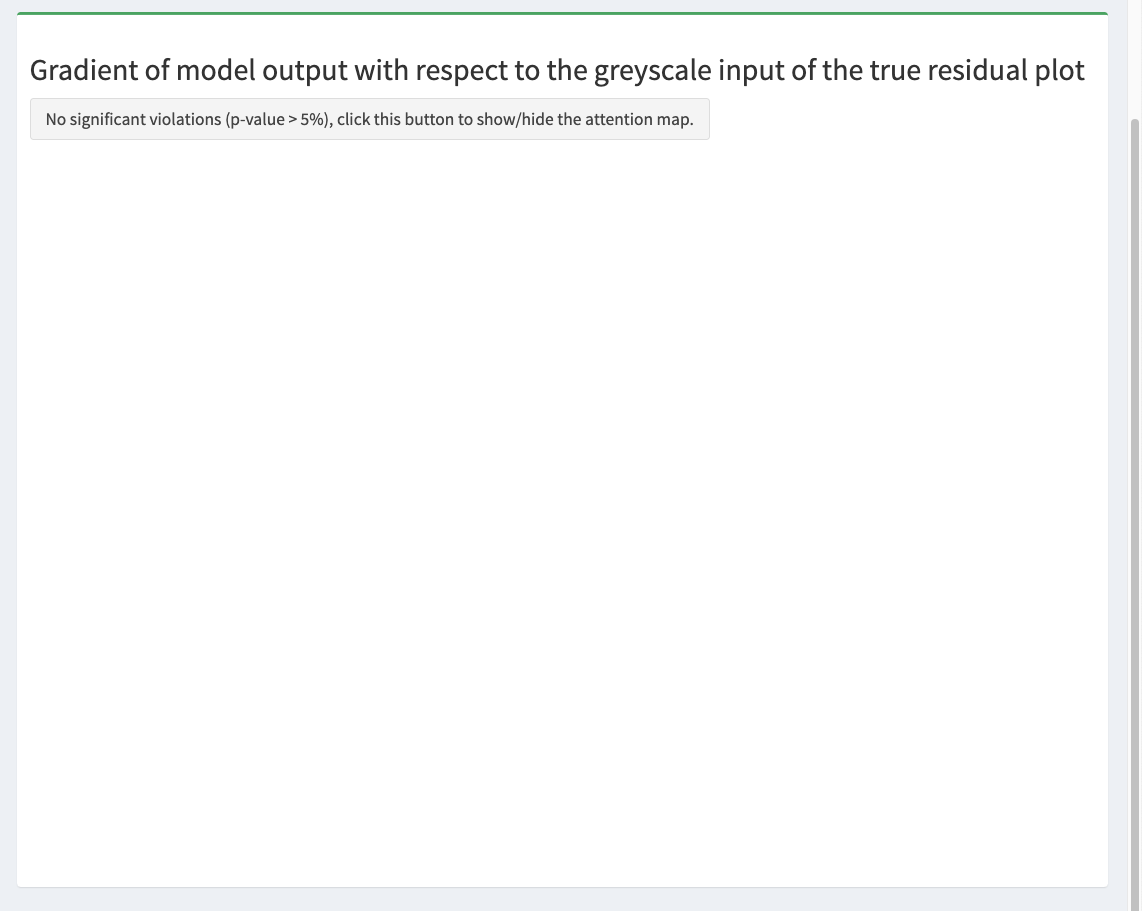
\includegraphics[width=0.5\linewidth,height=\textheight,keepaspectratio]{figures/autovi_web_gradient_hide.png}

}

\caption{\label{fig-autovi-web-gradient-hide}The attention map is hidden
if the assessment indicates a \(p\)-value greater than 0.05. A button is
available to toggle the display of the attention map.}

\end{figure}%

Region 6 of Figure~\ref{fig-autovi-web-result} contains an interactive
table created with the R package \texttt{DT} \citep{dt}, which provides
the VSS. This table includes four columns: \texttt{.sample},
\texttt{vss}, \texttt{rank}, and \texttt{null}. The \texttt{.sample}
column shows the residual plot labels. For a CSV type that is a lineup,
these labels are taken from an identifier column in the dataset
specified by the user. In the case of the CSV type is a single residual
plot, labels are automatically generated from 1 to 20, with the true
residual plot receiving a randomly assigned label. The \texttt{vss}
column displays the VSS for each residual plot, rounded to three decimal
places. The \texttt{rank} column indicates the ranking of each residual
plot based on VSS. The \texttt{null} column reveals whether the plot is
a null plot. For the CSV type that is a single residual plot, only the
true residual plot will have ``false'' in this column, while all other
plots will be marked ``true.'' For the CSV type that is a lineup, if the
true residual plot identifier has not been provided, this column will
show ``NA'' to represent missing values. If the identifier is provided
by user, the column behaves as if the CSV type is a single residual
plot.

The \texttt{DT} table provides several interactive features. Users can
download the table in four formats, including text, CSV, Excel, and PDF,
using the buttons located above the table. Additionally, the table is
searchable via the text input field also positioned above it. Below the
table, a text message displays the \(p\)-value of the assessment for the
true residual plot and summarizes the number of null plots with VSS
greater than that of the true residual plot. This helps the user
determine whether the true residual plot shows visual patterns that
suggest model violations.

Region 7 of Figure~\ref{fig-autovi-web-result} provides a lineup of
plots corresponding to each \texttt{.sample} value from the table in
Region 6. Due to space limitations, a maximum of 20 residual plots will
be displayed, ensuring that the true residual plot, if known, will be
included in the lineup. The plots are generated using \texttt{ggplot2},
the same as in \texttt{autovi}. Users can perform a visual test with
this lineup to check if the true residual plot is distinguishable from
the other plots, helping to determine the significance of model
violations.

Region 8 of Figure~\ref{fig-autovi-web-result2} displays the density
plot for bootstrapped VSS and null VSS. The densities are shown in
distinct colors that are friendly for colorblind users. A solid vertical
line marks the VSS of the true residual plot, while rug lines at the
bottom of the plot provide a clearer view of individual cases. Below the
plot, a text message indicates the number and percentage of bootstrapped
residual plots that would be rejected by the visual test when compared
to the null plots. Note that the bootstrapped residual plots in this
application are generated differently from \texttt{autovi}. Since we do
not have the R model object, we can not refit the regression model with
bootstrapped data. Instead, we bootstrap the residuals of the true
residual plot directly to obtain bootstrapped residual plots. As as
result, this panel will disappear when the true residual plot is
unknown.

Region 9 of Figure~\ref{fig-autovi-web-result2} displays an attention
map for the true residual plot, generated by computing the gradient of
the Keras model's output with respect to the greyscale input of the
plot. The attention map helps to understand how the Keras model predicts
VSS and which areas it is focusing on. We use a greyscale input because
it is easier to generate a clear attention map in this format, and it
usually conveys all the essential information, as most of the important
details of the plot are drawn in black. If the \(p\)-value of the true
residual plot is greater than 0.05, checking the attention map is not
necessary. However, to provide users with the option to review it if
they wish, a button will be available, as shown in
Figure~\ref{fig-autovi-web-gradient-hide}. This button allows users to
toggle the display of the attention map.

\subsection{Workflow}\label{sec-autovi-web-workflow}

The workflow of \texttt{autovi.web} is designed to be straightforward,
with numbered steps displayed in each panel shown in
Figure~\ref{fig-autovi-web}. There are two example datasets provided by
the web application, as mentioned in
Section~\ref{sec-autovi-web-design}. The single residual plot example
uses the \texttt{dino} dataset from the R package \texttt{datasauRus}
\citep{datasaurus}. The lineup example uses residuals from a simulated
regression model that has a non-linearity issue. We will walk through
the lineup example to further demonstrate the workflow of the web
application.

As shown in Figure~\ref{fig-autovi-web-workflow-example1}, to use the
lineup example data, click the ``Use Lineup Example'' button. The data
status will then update to show the number of rows and columns in the
dataset, and the CSV type will automatically be selected to the correct
option. Since the example dataset follows the variable naming
conventions assumed by the web application, the columns for fitted
values, residuals, and labels of residual plots are set automatically
(Figure~\ref{fig-autovi-web-workflow-example2}). If the user is working
with a custom dataset, these options must be set accordingly. Regardless
of the dataset, the user must manually select the label for the true
residual plot, as the web application allows assessments without this
label. The next step is to click the play button to start the
assessment.

Results are provided in multiple panels as displayed in
Figure~\ref{fig-autovi-web-workflow-example3},
Figure~\ref{fig-autovi-web-workflow-example4},
Figure~\ref{fig-autovi-web-workflow-example5} and
Figure~\ref{fig-autovi-web-workflow-example6}. In
Figure~\ref{fig-autovi-web-workflow-example3}, the first row of the
table is the most crucial to check, as it provides the VSS and the rank
of the true residual plot among the other plots. The summary text
beneath the table provides the \(p\)-value, which can be used for quick
decision-making. In Figure~\ref{fig-autovi-web-workflow-example4}, the
lineup is for manual inspection, and the user should see if the true
residual plot is visually distinguishable from the other plots, to
confirm if the model violation is serious. The density plot in
Figure~\ref{fig-autovi-web-workflow-example5} offers a more robust
result, allowing the user to compare the distribution of bootstrapped
VSS with the distribution of null VSS. Finally, the grayscale attention
map shown in Figure~\ref{fig-autovi-web-workflow-example6} can be used
to check if the target visual features, like the non-linearity present
in the lineup example, are captured by the computer vision model,
ensuring the quality of the assessment.

\begin{figure}

\centering{

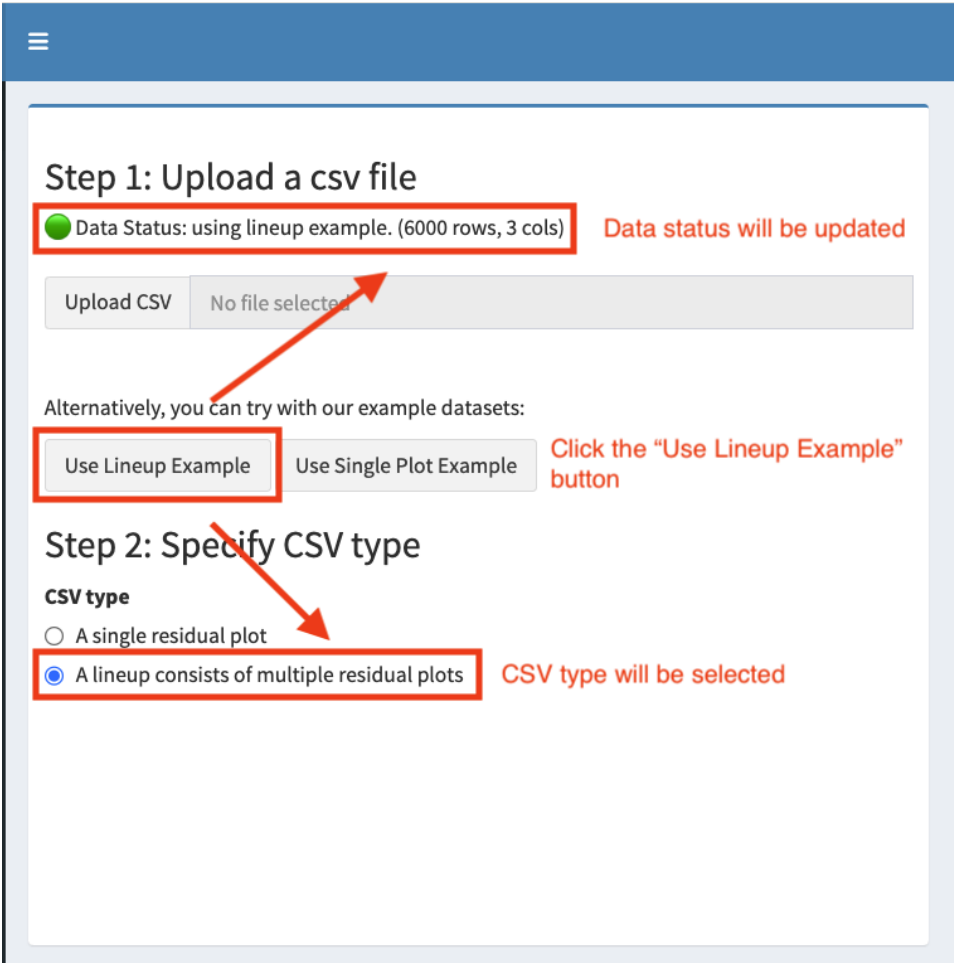
\includegraphics[width=0.8\linewidth,height=\textheight,keepaspectratio]{autovi_paper_files/figure-pdf/fig-autovi-web-workflow-example1-1.png}

}

\caption{\label{fig-autovi-web-workflow-example1}To begin the workflow
for \texttt{autovi} using the lineup example dataset, the user clicks
the ``Use Lineup Example'' button to load the example dataset, during
which the data status and CSV type will be automatically updated.}

\end{figure}%

\begin{figure}

\centering{

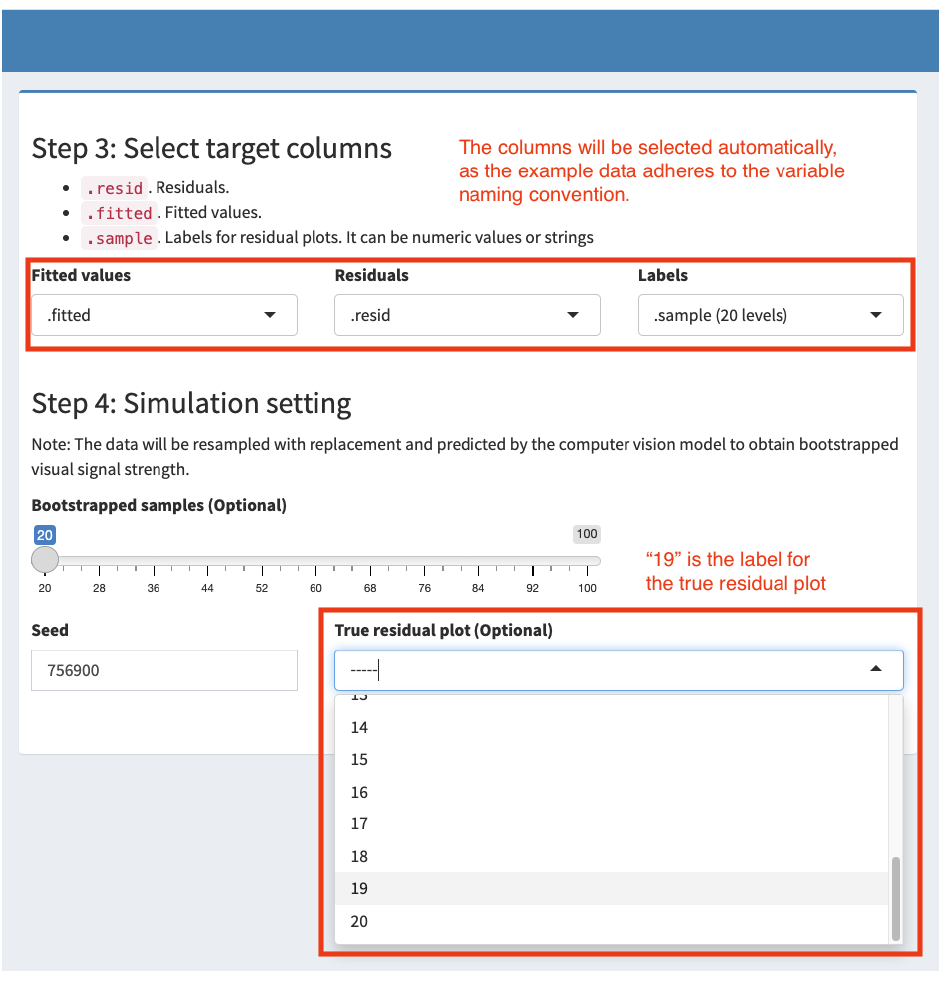
\includegraphics[width=0.8\linewidth,height=\textheight,keepaspectratio]{autovi_paper_files/figure-pdf/fig-autovi-web-workflow-example2-1.png}

}

\caption{\label{fig-autovi-web-workflow-example2}After clicking the
button in Figure~\ref{fig-autovi-web-workflow-example1}, the target
columns are selected automatically, though the user must manually select
the label for the true residual plot, as the web application permits
assessment without this label.}

\end{figure}%

\begin{figure}

\centering{

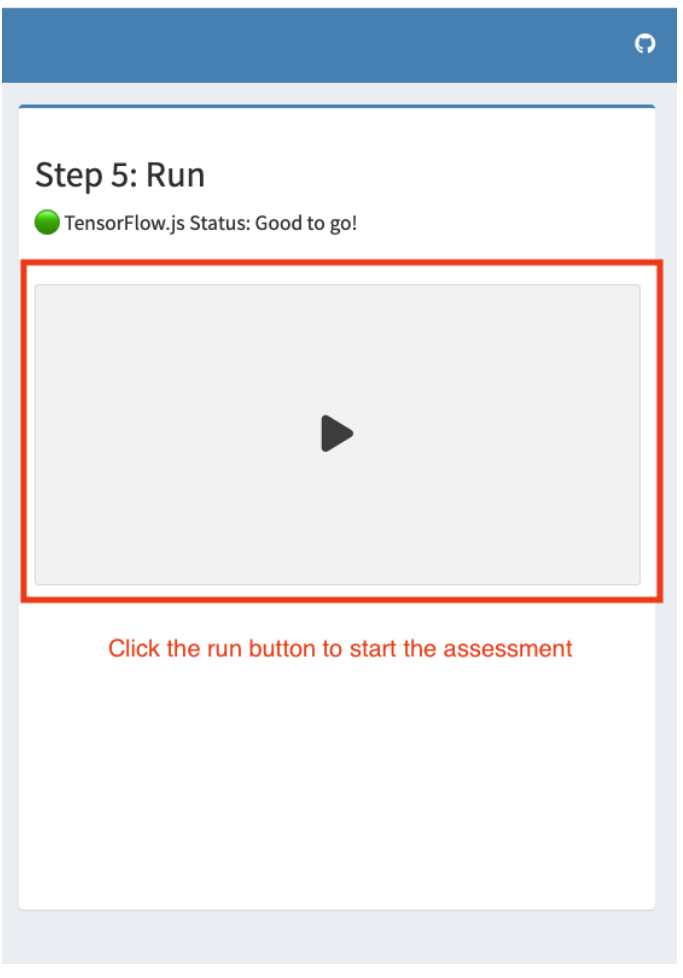
\includegraphics[width=0.55\linewidth,height=\textheight,keepaspectratio]{autovi_paper_files/figure-pdf/fig-autovi-web-workflow-example3-1.png}

}

\caption{\label{fig-autovi-web-workflow-example3}After finishing the
required steps in Figure~\ref{fig-autovi-web-workflow-example1} and
Figure~\ref{fig-autovi-web-workflow-example2}, the user initiates the
assessment of the lineup example data by clicking the run button.}

\end{figure}%

\begin{figure}

\centering{

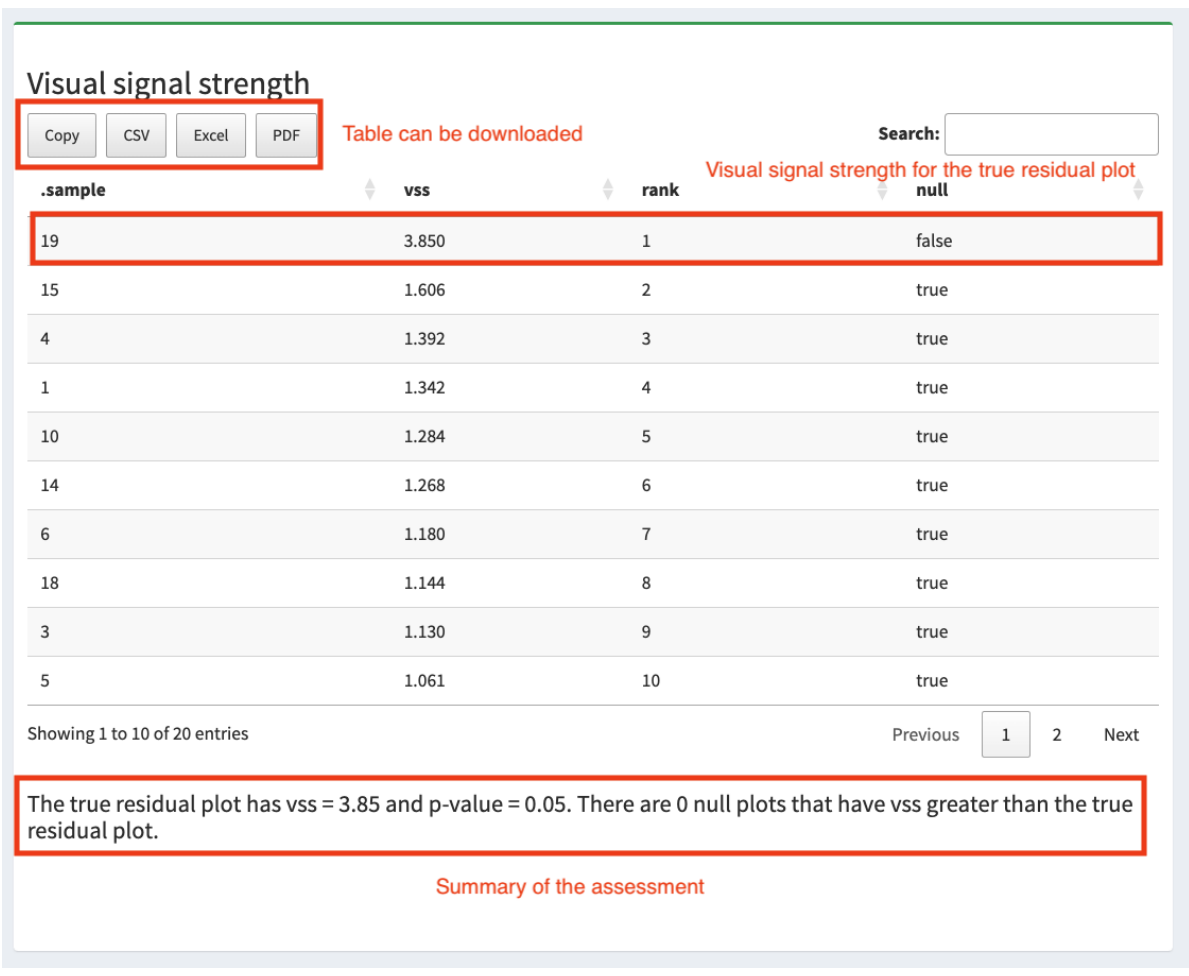
\includegraphics[width=1\linewidth,height=\textheight,keepaspectratio]{autovi_paper_files/figure-pdf/fig-autovi-web-workflow-example4-1.png}

}

\caption{\label{fig-autovi-web-workflow-example4}The VSS of the true
residual plot is displayed in the first row of the table, with a summary
text beneath the table providing the \(p\)-value to aid in
decision-making.}

\end{figure}%

\begin{figure}

\centering{

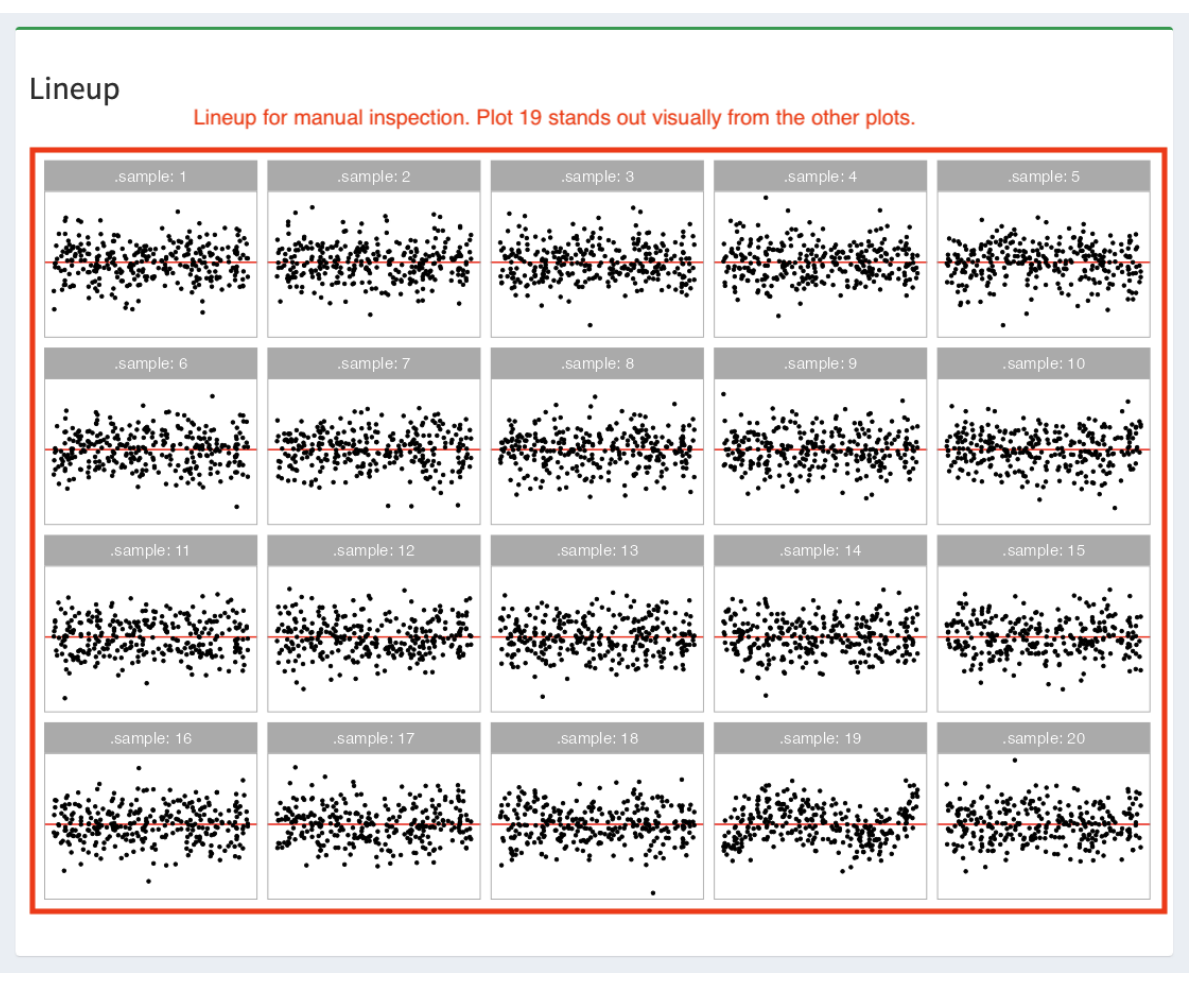
\includegraphics[width=1\linewidth,height=\textheight,keepaspectratio]{autovi_paper_files/figure-pdf/fig-autovi-web-workflow-example5-1.png}

}

\caption{\label{fig-autovi-web-workflow-example5}A lineup of residual
plots allows for manual inspection.}

\end{figure}%

\begin{figure}

\centering{

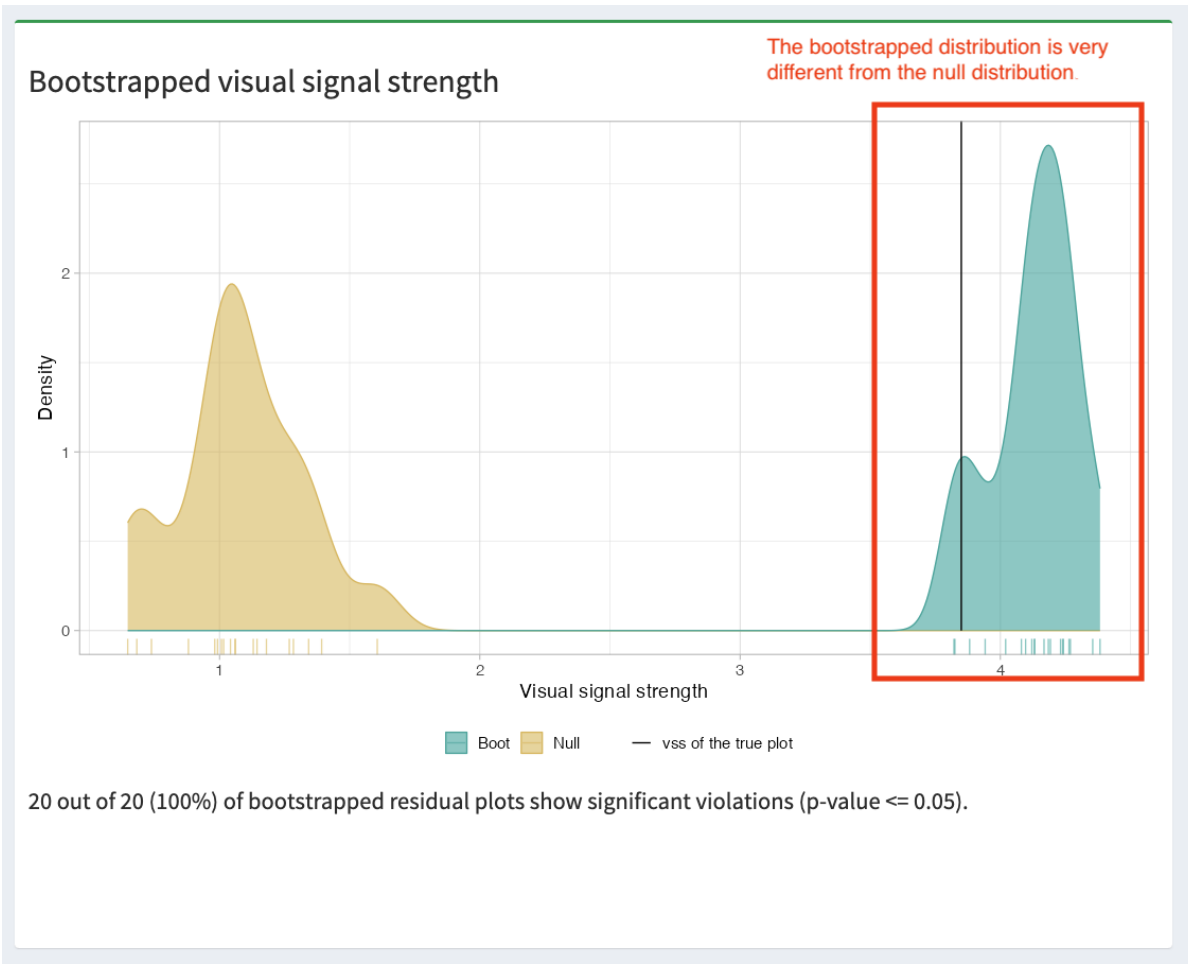
\includegraphics[width=1\linewidth,height=\textheight,keepaspectratio]{autovi_paper_files/figure-pdf/fig-autovi-web-workflow-example6-1.png}

}

\caption{\label{fig-autovi-web-workflow-example6}The density plot helps
verify if the bootstrapped distribution differs from the null
distribution.}

\end{figure}%

\begin{figure}

\centering{

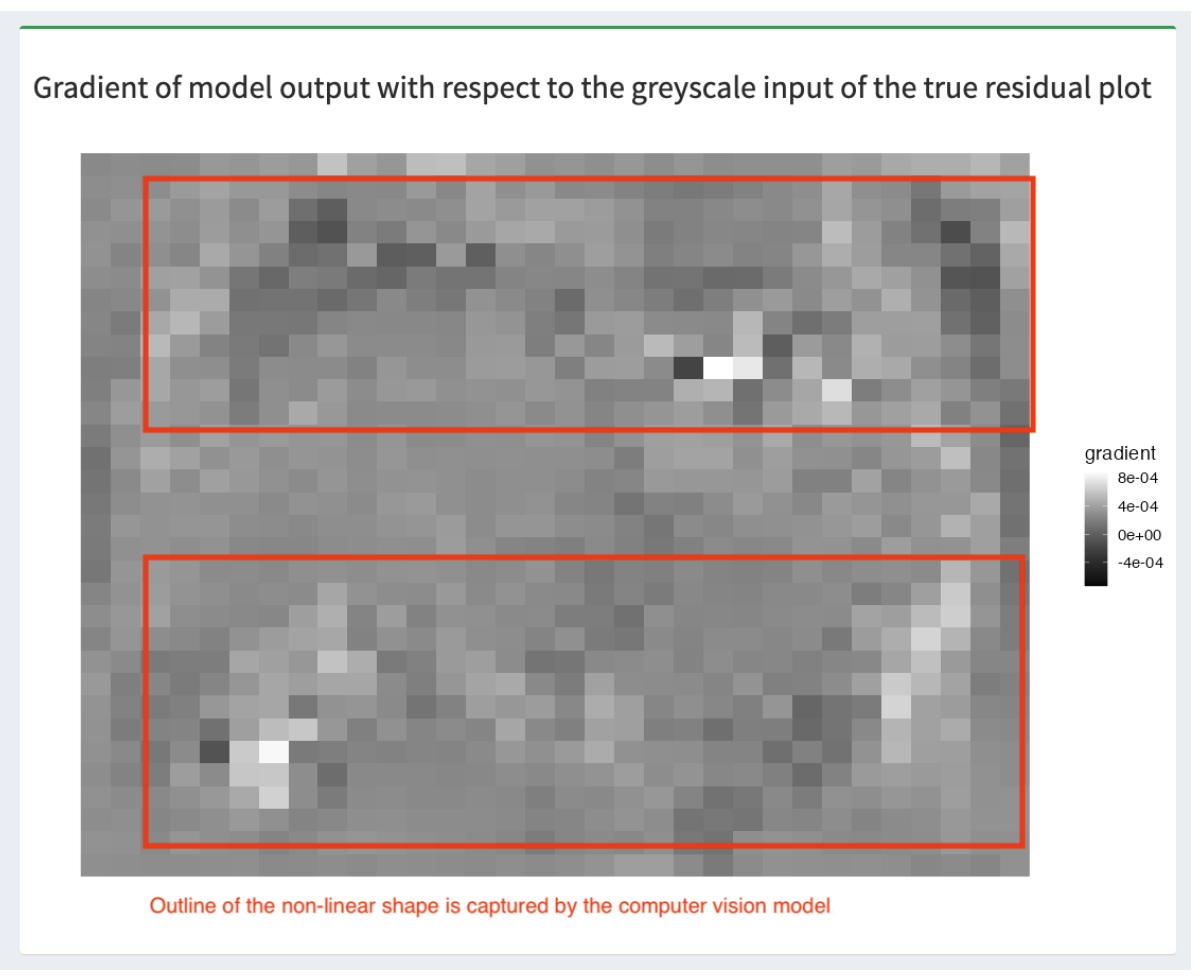
\includegraphics[width=1\linewidth,height=\textheight,keepaspectratio]{autovi_paper_files/figure-pdf/fig-autovi-web-workflow-example7-1.png}

}

\caption{\label{fig-autovi-web-workflow-example7}The attention map
offers insights into whether the computer vision model has captured the
intended visual features of the true residual plot.}

\end{figure}%

\section{Conclusions}\label{sec-autovi-conclusion}

This paper presents new regression diagnostics software, the R package
\texttt{autovi} and its accompanying web interface package,
\texttt{autovi.web}. It addresses a critical gap in the current
landscape of statistical software. While regression tools are widely
available, effective and efficient diagnostic methods have lagged
behind, particularly in the field of residual plot interpretation.

The \texttt{autovi} R package, introduced in this paper, automates the
assessment of residual plots by incorporating a computer vision model,
eliminating the need for time-consuming and potentially inconsistent
human interpretation. This automation improves the efficiency of the
diagnostic process and promotes consistency in model evaluation across
different users and studies.

The development of the accompanying Shiny app, \texttt{autovi.web},
expands access to these advanced diagnostic tools, by providing a
user-friendly interface. It makes automated residual plot assessment
accessible to a broader audience, including those who may not have
extensive programming experience. This web-based solution effectively
addresses the potential barriers to adoption, such as complex
dependencies and installation requirements, that are often associated
with advanced statistical software.

The combination of \texttt{autovi} and \texttt{autovi.web} offers a
comprehensive solution to the challenges of residual plot interpretation
in regression analysis. These tools have the potential to significantly
improve the quality and consistency of model diagnostics across various
fields, from academic research to industry applications. By automating a
critical aspect of model evaluation, they allow researchers and analysts
to focus more on interpreting results and refining models, rather than
grappling with the intricacies of plot assessment.

The framework established by \texttt{autovi} and \texttt{autovi.web}
opens up exciting possibilities for further research and development.
Future work could explore the extension of these automated assessment
techniques to other types of diagnostic plots and statistical models,
potentially revolutionizing how we approach statistical inference using
visual displays more broadly.

\section{Resources and Supplementary
Material}\label{resources-and-supplementary-material}

The the current version of \texttt{autovi} can be installed from CRAN,
and source code for both packages are available at
\url{https://github.com/TengMCing/autovi}. The web interface is
available from \url{autoviweb.netlify.app}.

These \texttt{R} packages were used for the work: \texttt{tidyverse}
\citep{tidyverse}, \texttt{lmtest} \citep{lmtest}, \texttt{kableExtra}
\citep{kableextra}, \texttt{patchwork} \citep{patchwork},
\texttt{rcartocolor} \citep{rcartocolor}, \texttt{glue} \citep{glue},
\texttt{here} \citep{here}, \texttt{magick} \citep{magick},
\texttt{yardstick} \citep{yardstick} and \texttt{reticulate}
\citep{reticulate}.


  \bibliography{bibliography.bib}



\end{document}
